% !LW recipe = XeLaTeX once (current file)
\ifdefined\CourseRootDocument
\providecommand{\FinishStandaloneChapter}{}
\else
\documentclass[11pt,oneside,openany,UTF8,fontset=none]{ctexbook}
\def\StandaloneChapterNumber{1}
\def\StandaloneCourseSetup{\UseMacroICourse}
% 单章/单附录构建前导区。
% 文档类声明保留在源文件中，便于 LaTeX Workshop 将当前文件识别为根文件；
% 本文件只补充共享前导区和正文环境。

% 单文件配方以源文件所在目录为工作目录；将项目根目录加入搜索路径，
% 因而文件名可包含空格和中文，也无需写入绝对的 iCloud 路径。
\makeatletter
\def\input@path{{../../}}
\makeatother
\newcommand{\ProjectRootPath}{../..}

% 全项目共享前导区：集中声明依赖顺序，整书与单章只引用这一处
% 用户可调文件位于 _config/，实现文件位于 _config/core/
% !TeX root = ../AMaN_SUN.tex
% 项目基本信息。

\newcommand{\DocumentTitle}{Advanced Macroeconomics I \& II}
\newcommand{\DocumentVersion}{2nd edition}
\newcommand{\CourseContributor}{Rongqing SUN}
\newcommand{\CourseContributorEmail}{econsunrq@outlook.com}
\newcommand{\CourseInstitution}{{\color{InstitutionMark}Xiamen University}}
\newcommand{\CourseAffiliation}{%
    SOE\hspace{0.5em}\(\boldsymbol{\times}\)\hspace{0.5em}%
    WISE\hspace{0.5em}\(\boldsymbol{\times}\)\hspace{0.5em}CHOW%
}
\newcommand{\CourseLevel}{Graduate Program}
\newcommand{\CourseSideLevel}{Graduate}
\newcommand{\CoursePartAuthor}{\CourseContributor}
\newcommand{\CourseLicenseToken}{CC BY-NC 4.0}
\newcommand{\CoursePartDate}{\CourseCompileDate}
\newcommand{\CourseEmblem}{xmu-emblem.png}

% 主封面上的两册课程信息。
\newcommand{\CoverFirstTerm}{Fall 2026}
\newcommand{\CoverFirstInstructor}{Yinong TAN}
\newcommand{\CoverFirstTopic}{Economic Growth}
\newcommand{\CoverSecondTerm}{Spring 2026}
\newcommand{\CoverSecondInstructor}{Chengyuan HE}
\newcommand{\CoverSecondTopic}{Economic Fluctuation}

% 当前课程配置；课程切换时只更新实际被版式读取的字段。
\newcommand{\CourseVolumeRoman}{I}
\newcommand{\CourseShortTitle}{Adv Macro I}
\newcommand{\CourseTerm}{Fall 2026}
\newcommand{\CourseInstructor}{Yinong TAN}

% 编译日期。
\newcommand{\TwoDigitDatePart}[1]{\ifnum#1<10 0\fi\number#1}
\newcommand{\CourseCompileDate}{%
    \number\year-\TwoDigitDatePart{\month}-\TwoDigitDatePart{\day}%
}
\newcommand{\CourseSideInfo}{%
    \CourseShortTitle\sideinfosep\CourseSideLevel\sideinfosep
    \CourseTerm\sideinfosep\CourseInstructor\sideinfosep\CourseCompileDate
}

\newcommand{\UseSharedCourseCover}{%
    \renewcommand{\CourseShortTitle}{Adv Macro I \& II}%
    \setcourseaccent{VolumeOneAccent}%
}
\newcommand{\UseMacroICourse}{%
    \renewcommand{\CourseShortTitle}{Adv Macro I}%
    \renewcommand{\CourseTerm}{Fall 2026}%
    \renewcommand{\CourseInstructor}{Yinong TAN}%
    \renewcommand{\CourseVolumeRoman}{I}%
    \renewcommand{\CourseSideInfo}{%
        \CourseShortTitle\sideinfosep\CourseSideLevel\sideinfosep
        \CourseTerm\sideinfosep\CourseInstructor\sideinfosep\CourseCompileDate}%
    \setcourseaccent{VolumeOneAccent}%
}
\newcommand{\UseMacroIICourse}{%
    \renewcommand{\CourseShortTitle}{Adv Macro II}%
    \renewcommand{\CourseTerm}{Spring 2026}%
    \renewcommand{\CourseInstructor}{Chengyuan HE}%
    \renewcommand{\CourseVolumeRoman}{II}%
    \renewcommand{\CourseSideInfo}{%
        \CourseShortTitle\sideinfosep\CourseSideLevel\sideinfosep
        \CourseTerm\sideinfosep\CourseInstructor\sideinfosep\CourseCompileDate}%
    \setcourseaccent{VolumeTwoAccent}%
}
\newcommand{\UseAppendixCourse}{%
    \renewcommand{\CourseSideInfo}{%
        Notes on Adv MacroEcon I \& II\sideinfosep\CourseSideLevel\sideinfosep
        Appendix\sideinfosep\CourseCompileDate}%
    \setcourseaccent{AppendixAccent}%
}

% 参考文献开关；正文出现引用后再启用。
\newif\ifcoursebibliography
\coursebibliographyfalse

% !TeX root = ../AMaN_SUN.tex
% 主封面重要参数。没有单位的数值均表示 pt 字号。

% 顶部校徽模块：距页面顶部、校徽尺寸及图文水平距离。
% 文字以校徽的垂直中心定位，改变校徽尺寸时不需要重新调整文字高度。
\newcommand{\CoverIdentityTop}{22mm}
\newcommand{\CoverEmblemSize}{19mm}
\newcommand{\CoverEmblemTextGap}{6mm}
\newcommand{\CoverIdentityInstitutionSize}{14.5}
\newcommand{\CoverIdentityInstitutionLeading}{18}
\newcommand{\CoverIdentityAffiliationSize}{9.5}
\newcommand{\CoverIdentityAffiliationLeading}{12}
\newcommand{\CoverIdentityLevelSize}{10.5}
\newcommand{\CoverIdentityLevelLeading}{13}

% 右上角横向 AMaN Logo：与校徽模块共用顶边，与页面右侧网格对齐。
\newcommand{\CoverBrandLogoScale}{0.90}
\newcommand{\CoverBrandLogoTop}{\CoverIdentityTop}
\newcommand{\CoverBrandLogoRight}{\CoverGridLeftX}

% 主标题字号、行距，以及灰色辅助词的字号和行距。
\newcommand{\CoverTitleMainSize}{39}
\newcommand{\CoverTitleMainLeading}{38}
\newcommand{\CoverTitleMetaSize}{26}
\newcommand{\CoverTitleMetaLeading}{29}
\newcommand{\CoverTitleLineGap}{22pt}

% 两个学期课程模块的主题、学期和教师信息字号。
\newcommand{\CoverTopicSize}{22}
\newcommand{\CoverTermSize}{13}
\newcommand{\CoverInstructorSize}{12}

% 左侧统一网格：标题、II 的左边界与作者信息从第一列开始，课程文字从第二列开始。
\newcommand{\CoverGridLeftX}{24mm}
\newcommand{\CoverGridTextX}{52mm}

% 主标题与两个课程模块的位置；数值越大，位置越靠右或靠下。
\newcommand{\CoverTitleTop}{70mm}
\newcommand{\CoverModuleTextX}{\CoverGridTextX}
\newcommand{\CoverFirstModuleY}{140mm}
\newcommand{\CoverSecondModuleY}{190mm}
\newcommand{\CoverModuleLineStep}{8.5mm}

% TikZ 绘制的 I、II 的右边界、笔画粗细和 II 两笔之间的距离。
\newcommand{\CoverNumeralRightX}{40mm}
\newcommand{\CoverNumeralStrokeWidth}{5.5mm}
\newcommand{\CoverNumeralGap}{5mm}

% 底部作者与版本信息共用三条基线；两侧每一行始终等高。
\newcommand{\CoverFooterBottomY}{21mm}
\newcommand{\CoverFooterRowStep}{9mm}
\newcommand{\CoverFooterLabelSize}{10.5}
\newcommand{\CoverFooterMainSize}{16}

% !TeX root = ../AMaN_SUN.tex
% Part 封面重要参数。没有单位的数值均表示 pt 字号。

% 右侧色块中的 Part 编号、中英文标题字号。
\newcommand{\PartCoverNumberSize}{96}
\newcommand{\PartCoverChineseTitleSize}{28}
\newcommand{\PartCoverChineseTitleLeading}{31}
\newcommand{\PartCoverEnglishTitleSize}{16}
\newcommand{\PartCoverEnglishTitleLeading}{18}

% Part + 罗马数字作为一个整体的纵向位移；正值向下，负值向上。
\newcommand{\PartCoverPartBlockShift}{4mm}

% “Part”和罗马数字在该模块内部的位置。
\newcommand{\PartCoverLabelTop}{60mm}
\newcommand{\PartCoverNumberTop}{80mm}

% 中英文标题的顶部位置；与署名区共同拉开整页纵向节奏。
\newcommand{\PartCoverChineseTitleTop}{154mm}
\newcommand{\PartCoverEnglishTitleTop}{212mm}

% 右侧色块顶部的横向 AMaN Logo；与左侧校徽模块共用顶边和色块中心轴。
\newcommand{\PartCoverBrandLogoTop}{\CoverIdentityTop}
\newcommand{\PartCoverBrandLogoScale}{0.90}

% 右侧署名区距离：分别控制 Prepared by、作者名和版权信息的间隔。
\newcommand{\PartCoverPreparedTopGap}{27mm}
\newcommand{\PartCoverAuthorGap}{10mm}
\newcommand{\PartCoverLegalGap}{27mm}

% 左侧校徽模块的顶部位置；尺寸与字号完全复用主封面设置。
\newcommand{\PartCoverLeftTopSpace}{-8mm}
\newcommand{\PartCoverLeftHeight}{248mm}

% 左侧课程名称字号，以及校徽模块与课程名称之间的距离。
\newcommand{\PartCoverCourseSize}{20}
\newcommand{\PartCoverCourseLeading}{21}
\newcommand{\PartCoverCourseTopGap}{60pt}

% 左侧局部目录采用总目录的 footnotesize，并使用相同的 1.50 倍行距。
\newcommand{\PartCoverContentsLineStretch}{1.50}
% 每章前的附加留白，以当前目录行高为单位。
\newcommand{\PartCoverChapterGap}{0.82}

% !TeX root = ../AMaN_SUN.tex
% 全项目字体与字号的可调参数。

% Sidenote 的中文基准字号与行距。
\newcommand{\SidenoteBaseFontSize}{9.1pt}
\newcommand{\SidenoteBaseLeading}{11.6pt}

% Sidenote 内西文字体的缩放比例；不改变中文字号。
\newcommand{\SidenoteLatinScale}{0.90}

% Sidenote 内所有 \(...\) 公式相对于侧注字号的缩放比例。
\newcommand{\SidenoteMathScale}{0.95}

% !TeX root = ../../AMaN_SUN.tex
% Fonts and core typography.
\usepackage{iftex}
\ifPDFTeX
    \PackageError{AdvMacro Notes}{This project requires XeLaTeX}{}
\fi
\usepackage{fontspec}
\usepackage{xeCJK}
\IfFontExistsTF{Source Han Serif SC}
    {\setCJKmainfont{Source Han Serif SC}[
        BoldFont=Source Han Serif SC Bold,
        ItalicFont=Source Han Serif SC,
        ItalicFeatures={FakeSlant=0.18},
        BoldItalicFont=Source Han Serif SC Bold,
        BoldItalicFeatures={FakeSlant=0.18}
    ]}
    {\setCJKmainfont{Songti SC}}
\IfFontExistsTF{Source Han Sans SC}
    {\setCJKsansfont{Source Han Sans SC}[BoldFont=Source Han Sans SC Bold]\setCJKmonofont{Source Han Sans SC}}
    {\setCJKsansfont{Heiti SC}\setCJKmonofont{Heiti SC}}
\setCJKfamilyfont{notekai}{FandolKai-Regular.otf}[BoldFont=FandolKai-Regular.otf]
\providecommand{\kaiti}{}
\renewcommand{\kaiti}{\CJKfamily{notekai}}
\providecommand{\heiti}{}
\renewcommand{\heiti}{\sffamily}
\usepackage[scaled=1.02]{newpxtext}
\usepackage[protrusion=true,expansion=false]{microtype}
% 在中文标点被 newunicodechar 改成活动字符前载入 Palatino 配置；
% 否则 microtype 会把省略号和破折号宏误判为未知字体槽位。
\LoadMicrotypeFile{Palatino}

% Mathematics.
\usepackage{mathtools}
\usepackage{amsthm}
\usepackage{amssymb}
\usepackage{newpxmath}
\usepackage[scr=boondoxo]{mathalfa}
\usepackage{empheq}
\usepackage{bm}
\usepackage{scalerel}
\providecommand{\symbfit}[1]{\bm{#1}}

% Page and document structure.
\usepackage{geometry}
\usepackage{setspace}
\usepackage{needspace}
\usepackage{fancyhdr}
\usepackage{titlesec}
\usepackage[bottom]{footmisc}
\usepackage{marginnote}
\usepackage{etoc}

% Figures, tables, and diagrams.
\usepackage{graphicx}
\usepackage{float}
\usepackage{caption}
\usepackage{subcaption}
\usepackage{booktabs}
\usepackage{array}
\usepackage{tabularx}
\usepackage{longtable}
\usepackage{makecell}
\usepackage{multirow}
\usepackage{tikz}
\usetikzlibrary{arrows.meta}

% Lists, utilities, bibliography, and links.
\usepackage[dvipsnames]{xcolor}
\usepackage{enumitem}
\usepackage{xparse}
\usepackage{etoolbox}
\usepackage{xstring}
\usepackage{mfirstuc}
\usepackage{csquotes}
\ifcoursebibliography
    \usepackage[
        backend=biber,
        style=authoryear-comp,
        sorting=nyt,
        maxbibnames=99,
        giveninits=true,
        uniquename=init,
        dashed=false,
        natbib=true
    ]{biblatex}
    \addbibresource{references.bib}
\else
    \providecommand{\printbibliography}[1][]{}
\fi
\usepackage{hyperref}
\usepackage{bookmark}
\usepackage[nameinlink,noabbrev]{cleveref}

% !TeX root = ../../AMaN_SUN.tex
% 项目资源路径。正文插图可直接写文件名，例如：
% \includegraphics{chapter-10-irf.png}

% 主文档从项目根目录构建；独立 chapter/appendix 会在其前导区中覆盖此值。
\providecommand{\ProjectRootPath}{.}

% 仅保留经常使用的资源目录变量，避免正文散落硬编码路径。
\newcommand{\AssetRootPath}{\ProjectRootPath/_assets}
\newcommand{\FigurePath}{\AssetRootPath/figures}
\newcommand{\ImagePath}{\AssetRootPath/images}
\newcommand{\MatlabPath}{\AssetRootPath/matlab}

% 非图片资源可通过下面的命令拼接路径。
\newcommand{\AssetFile}[1]{\AssetRootPath/#1}
\newcommand{\FigureFile}[1]{\FigurePath/#1}
\newcommand{\ImageFile}[1]{\ImagePath/#1}
\newcommand{\MatlabFile}[1]{\MatlabPath/#1}

% graphicx 会依次在 figures 与 images 中查找，因此插图时只需写文件名。
\edef\CourseGraphicSearchPath{{\FigurePath/}{\ImagePath/}}
\expandafter\graphicspath\expandafter{\CourseGraphicSearchPath}

% !TeX root = ../AMaN_SUN.tex
% 全项目颜色统一定义。颜色名称只描述用途，不描述具体色相。

% 页面与文字层级。
\definecolor{PageBackground}{HTML}{FAF9F7}
\definecolor{BodyText}{HTML}{25272A}
\definecolor{SecondaryText}{HTML}{746F69}
\definecolor{Divider}{HTML}{D8D3CC}
\definecolor{InstitutionMark}{HTML}{003C88}
\definecolor{DiagramPrimary}{HTML}{25272A}
\definecolor{DiagramAnnotation}{HTML}{746F69}
\definecolor{DiagramGuide}{HTML}{999793}
\definecolor{PartPrimaryText}{HTML}{FAF9F7}

% 两册课程主题色：第一册为马卡龙橙，第二册为马卡龙绿。
\definecolor{VolumeOneAccent}{HTML}{C98256}
\definecolor{VolumeTwoAccent}{HTML}{74A184}
\definecolor{AppendixAccent}{HTML}{867dab}
\definecolor{MathEmphasisB}{HTML}{477695}
\definecolor{MathEmphasisC}{HTML}{ae7992}

% 当前课程及其派生用途。切换课程时同步更新。
\colorlet{ActiveAccent}{VolumeOneAccent}
\colorlet{MathEmphasisA}{VolumeOneAccent}
\colorlet{MathEmphasisB}{VolumeTwoAccent}
\colorlet{MathEmphasisC}{AppendixAccent}
\colorlet{DiagramHighlight}{ActiveAccent}
\colorlet{DiagramComparison}{ActiveAccent!48!BodyText}
\colorlet{PartSecondaryText}{PageBackground!72!ActiveAccent}

\newcommand{\setcourseaccent}[1]{%
    \colorlet{ActiveAccent}{#1}%
    \colorlet{MathEmphasisA}{ActiveAccent}%
    \colorlet{DiagramHighlight}{ActiveAccent}%
    \colorlet{DiagramComparison}{ActiveAccent!48!BodyText}%
    \colorlet{PartSecondaryText}{PageBackground!72!ActiveAccent}%
}

% !TeX root = ../AMaN_SUN.tex
% 全项目通用可调设置；不限于数学排版。

% 正文段间距；目录等紧凑区域可在局部覆盖。
\newlength{\BodyParagraphSpacing}
\setlength{\BodyParagraphSpacing}{3ex plus 0.3ex minus 0.2ex}

% 公式局部强调。
% Highlight：行内/行间公式分别设置横向、纵向内边距；浓度取值为 0--100。
\newlength{\MathHighlightInlineHorizontalPadding}
\setlength{\MathHighlightInlineHorizontalPadding}{3.2pt}
\newlength{\MathHighlightInlineVerticalPadding}
\setlength{\MathHighlightInlineVerticalPadding}{2.2pt}

\newlength{\MathHighlightDisplayHorizontalPadding}
\setlength{\MathHighlightDisplayHorizontalPadding}{4pt}
\newlength{\MathHighlightDisplayVerticalPadding}
\setlength{\MathHighlightDisplayVerticalPadding}{3.5pt}
\newcommand{\MathHighlightTint}{16}

% Frame：行内/行间公式分别设置横向、纵向内边距，并共用边框粗细。
\newlength{\MathFrameInlineHorizontalPadding}
\setlength{\MathFrameInlineHorizontalPadding}{1.2pt}
\newlength{\MathFrameInlineVerticalPadding}
\setlength{\MathFrameInlineVerticalPadding}{1pt}

\newlength{\MathFrameDisplayHorizontalPadding}
\setlength{\MathFrameDisplayHorizontalPadding}{1.6pt}
\newlength{\MathFrameDisplayVerticalPadding}
\setlength{\MathFrameDisplayVerticalPadding}{2pt}
\newlength{\MathFrameRuleWidth}
\setlength{\MathFrameRuleWidth}{0.65pt}

% 全局等号颜色。
\definecolor{MathEqualsColor}{HTML}{909090}

% !TeX root = ../../AMaN_SUN.tex
% 数学排版实现；用户可调参数统一放在 _config/setting-general.tex。

\begingroup
    \catcode61=13
    \gdef={\mathrel{\color{MathEqualsColor}\mathchar"003D}}
\endgroup
\AtBeginDocument{\mathcode61="8000}

% !TeX root = ../../AMaN_SUN.tex
\color{BodyText}
\tikzset{every picture/.append style={color=DiagramPrimary}}
\AtBeginDocument{\pagecolor{PageBackground}}

% 主封面与 Part 封面只引用 Logo 总入口。
\def\LogoRootPath{logo}
\input{logo/logo}
\newsavebox{\AdvMacroBrandLogoBox}
\newsavebox{\CourseIdentityBox}

% 主封面与 Part 封面共用同一套校徽、字号、行距和图文间距。
\newcommand{\CourseIdentityGraphic}[1]{%
    \begin{tikzpicture}[baseline=(course-identity-text.base)]
        \node[anchor=west,inner sep=0pt] (course-emblem) at (0,0)
            {\includegraphics[width=\CoverEmblemSize]{\CourseEmblem}};
        \node[anchor=west,inner sep=0pt,text width=56mm,align=left]
            (course-identity-text) at ([xshift=\CoverEmblemTextGap]course-emblem.east)
            {{\HeadingLatinFont\fontsize{\CoverIdentityInstitutionSize}{\CoverIdentityInstitutionLeading}\selectfont\bfseries\CourseInstitution}\\[-1pt]
             {\HeadingLatinFont\fontsize{\CoverIdentityAffiliationSize}{\CoverIdentityAffiliationLeading}\selectfont\bfseries\color{#1}\CourseAffiliation}\\[-1pt]
             {\HeadingLatinFont\fontsize{\CoverIdentityLevelSize}{\CoverIdentityLevelLeading}\selectfont\color{SecondaryText}\CourseLevel}};
    \end{tikzpicture}%
}

\newlength{\SideMargin}
\setlength{\SideMargin}{22mm}
\newlength{\SymmetricMargin}
\setlength{\SymmetricMargin}{30mm}
\newlength{\MarginNoteWidth}
\setlength{\MarginNoteWidth}{35mm}
\newlength{\MarginNoteSep}
\setlength{\MarginNoteSep}{6mm}
\geometry{
    a4paper,
    left=\SideMargin,
    right=50mm,
    top=25mm,
    bottom=25mm,
    marginparwidth=\MarginNoteWidth,
    marginparsep=\MarginNoteSep,
    headheight=15pt,
    headsep=7mm,
    footskip=11mm
}
\newcommand{\notesymmetriclayout}{%
    \newgeometry{
        left=\SymmetricMargin,
        right=\SymmetricMargin,
        top=25mm,
        bottom=25mm,
        headheight=15pt,
        headsep=7mm,
        footskip=11mm
    }%
}
\newcommand{\notemainlayout}{\restoregeometry}
\normalmarginpar
\setlength{\marginparpush}{8pt}
\raggedbottom
% 浮动体在当前位置放不下时应延后排版，让后续正文继续填充本页。
% 跨页表格仍使用 longtable；普通 figure/table 不使用强制定位 [H]。
\setcounter{topnumber}{3}
\setcounter{bottomnumber}{2}
\setcounter{totalnumber}{5}
\renewcommand{\topfraction}{0.90}
\renewcommand{\bottomfraction}{0.80}
\renewcommand{\textfraction}{0.08}
\renewcommand{\floatpagefraction}{0.78}
\floatplacement{figure}{!htbp}
\floatplacement{table}{!htbp}
\setstretch{1.38}
\setlength{\parindent}{2em}
\setlength{\parskip}{2ex plus 0.3ex minus 0.2ex}
\newcommand{\TTTFont}{\fontsize{11.5pt}{12.5pt}\selectfont\ttfamily}
\DeclareRobustCommand{\ttt}[1]{{\TTTFont #1}}

\hypersetup{
    colorlinks=true,
    linkcolor=ActiveAccent,
    citecolor=ActiveAccent,
    urlcolor=ActiveAccent,
    bookmarksnumbered=true,
    bookmarksopen=true,
    bookmarksopenlevel=2,
    pdfstartview=FitH,
    pdftitle={\DocumentTitle},
    pdfauthor={\CourseContributor},
    pdfsubject={Advanced Macroeconomics}
}
\renewcommand{\UrlFont}{\TTTFont}

% Footer and left page-edge metadata.
\newif\ifnotesideinfo
\notesideinfofalse
\newcommand{\sideinfosep}{\quad{\color{Divider}/}\quad}
\fancypagestyle{notefancy}{%
    \fancyhf{}%
    \fancyhead[L]{{\normalfont\mdseries\small\color{SecondaryText}\nouppercase{\rightmark}}}%
    \fancyfoot[L]{{\normalfont\mdseries\small\color{SecondaryText}\thepage}}%
    \renewcommand{\headrulewidth}{0.3pt}%
    \renewcommand{\footrulewidth}{0pt}%
}
\fancypagestyle{plain}{%
    \fancyhf{}%
    \fancyfoot[L]{\ifnotesideinfo{\normalfont\mdseries\small\color{SecondaryText}\thepage}\fi}%
    \fancyfoot[C]{\ifnotesideinfo\else{\normalfont\mdseries\small\color{SecondaryText}\thepage}\fi}%
    \renewcommand{\headrulewidth}{0pt}%
    \renewcommand{\footrulewidth}{0pt}%
}
\fancypagestyle{symplain}{%
    \fancyhf{}%
    \fancyfoot[C]{{\normalfont\mdseries\small\color{SecondaryText}\thepage}}%
    \renewcommand{\headrulewidth}{0pt}%
    \renewcommand{\footrulewidth}{0pt}%
}
\AddToHook{shipout/foreground}{%
    \ifnotesideinfo
        \begin{tikzpicture}[remember picture,overlay]
            \node[
                rotate=90,
                anchor=center,
                font=\normalfont\mdseries\small,
                text=SecondaryText
            ] at ([xshift=10mm]current page.west)
            {\CourseSideInfo};
        \end{tikzpicture}%
    \fi
}

% Margin notes stay in the right margin on every page.
\newcommand{\SidenoteScaleMath}[1]{\scalebox{\SidenoteMathScale}{#1}}
% 在内容进入 marginnote 前，把每组 \(...\) 改写成完整且平衡的缩放组。
% 这样用户只需正常输入 \sidenote{文字 \(公式\) 文字}。
\ExplSyntaxOn
\cs_new_protected:Npn \sidenote_process_math:n #1
  {
    \tl_set:Nn \l_tmpa_tl {#1}
    \regex_replace_all:nnN
      { \c{\(} (.*?) \c{\)} }
      { \c{SidenoteScaleMath} \cB\{ \c{(} \1 \c{)} \cE\} }
      \l_tmpa_tl
    \tl_use:N \l_tmpa_tl
  }
\cs_new_eq:NN \SidenoteProcessMath \sidenote_process_math:n
\ExplSyntaxOff
\newfontfamily\SidenoteLatinFont{TeXGyrePagellaX}[Scale=\SidenoteLatinScale]
\newcommand{\SidenoteFont}{%
    \fontsize{\SidenoteBaseFontSize}{\SidenoteBaseLeading}\selectfont
    \SidenoteLatinFont
}
% Distinct styling for proper nouns or named concepts inside a margin note.
% Inherit the surrounding sidenote's size and leading.  Re-applying
% \SidenoteFont inside a CJK family switch makes XeCJK reset the glyphs to a
% smaller nominal size, so only the Kai family and active emphasis are changed.
\newcommand{\sidenoteterm}[1]{{\kaiti\color{ActiveAccent}#1}}
\let\sideterm\sidenoteterm
\newcommand{\sidenote}[1]{%
    \marginnote{%
        \raggedright
        \kaiti
        % 先选中文楷体，再应用西文字体与字号，避免西文 Scale 被覆盖。
        \SidenoteFont
        \setstretch{1.08}%
        \color{SecondaryText}%
        \SidenoteProcessMath{#1}%
    }%
}

% Numbered chapter openers show only the large Arabic numeral. The local
% clearing below does not alter CTeX's Chinese chapter label in the TOC.
\makeatletter
\newcommand{\chapterbodynumberonly}{%
    \let\CTEX@prechapter\@empty
    \let\CTEX@postchapter\@empty
}
\makeatother
\IfFontExistsTF{Source Han Sans SC}
    {\newfontfamily\HeadingLatinFont{Source Han Sans SC}[BoldFont=Source Han Sans SC Bold]}
    {\newcommand{\HeadingLatinFont}{\sffamily}}
\IfFontExistsTF{Source Han Sans SC Heavy}
    {\newfontfamily\CoverDisplayFont{Source Han Sans SC Heavy}}
    {\newcommand{\CoverDisplayFont}{\HeadingLatinFont\bfseries}}
\ctexset{
    chapter={
        name={第,章},
        number=\arabic{chapter},
        format=\normalfont\HeadingLatinFont\CJKfamily{\CJKsfdefault}\raggedleft,
        nameformat=\chapterbodynumberonly,
        numberformat=\fontsize{82}{76}\selectfont\HeadingLatinFont\CJKfamily{\CJKsfdefault}\bfseries\color{ActiveAccent},
        titleformat=\HeadingLatinFont\CJKfamily{\CJKsfdefault}\LARGE\bfseries\color{BodyText},
        aftername=\par\vspace{-3pt},
        beforeskip=8pt,
        afterskip=28pt
    }
}
\titleformat{\section}[block]
    {\normalfont\HeadingLatinFont\CJKfamily{\CJKsfdefault}\Large\bfseries\color{ActiveAccent}\raggedright}
    {\thesection}
    {0.8em}
    {}
\titleformat{\subsection}[block]
    {\normalfont\HeadingLatinFont\CJKfamily{\CJKsfdefault}\large\bfseries\color{ActiveAccent!82!BodyText}\raggedright}
    {\thesubsection}
    {0.8em}
    {}
\titleformat{\subsubsection}[block]
    {\normalfont\HeadingLatinFont\CJKfamily{\CJKsfdefault}\normalsize\bfseries\color{BodyText}\raggedright}
    {\textcolor{ActiveAccent}{\thesubsubsection}}
    {0.8em}
    {}
\titlespacing*{\section}{0pt}{18pt}{9pt}
\titlespacing*{\subsection}{0pt}{13pt}{6pt}
\titlespacing*{\subsubsection}{0pt}{10pt}{4pt}

% Classic main contents, matching the original project's standard dotted
% layout. Keep the whole-book directory compact independently from the
% larger directory printed on each Part opener.
\makeatletter
\newcommand{\GlobalTOCLineStretch}{1.50}
% Increase this value to open up the Part-local directory. This is deliberately
% separate from the global directory so the two layouts can be tuned alone.
\newcommand{\MainTOCLineStretch}{1.50}
\newcommand{\makecompacttableofcontents}{%
    \begingroup
    \footnotesize
    \etocstandardlines
    \etocsetnexttocdepth{section}% omit subsection (x.x.x) entries
    \setstretch{\GlobalTOCLineStretch}%
    \setlength{\parskip}{0pt}%
    \renewcommand{\@pnumwidth}{2.6em}% accommodate three-digit sans-serif page numbers
    \color{ActiveAccent}%
    % Switch only CJK glyphs to Source Han Sans; keep the Latin/math font
    % unchanged so raw Greek symbols in titles retain their existing glyphs.
    \HeadingLatinFont\CJKfamily{\CJKsfdefault}
    % LaTeX 的标准目录命令会对页码执行 \normalfont；这里仅覆盖页码字体，
    % 不改变总目录原有的缩进、点线和行距。
    \let\CourseOriginalDottedTocLine\@dottedtocline
    \renewcommand{\@dottedtocline}[5]{%
        \CourseOriginalDottedTocLine{##1}{##2}{##3}{##4}{{\HeadingLatinFont ##5}}}%
    \renewcommand*\l@part[2]{%
        \addpenalty{-\@highpenalty}%
        \addvspace{1.25em plus 1pt}%
        \begingroup
        \large\bfseries
        \noindent
        \makebox[\linewidth][c]{##1}% centered Part title
        \llap{\hb@xt@\@pnumwidth{\hss {\HeadingLatinFont ##2}}}% page number at right
        \par
        \endgroup
    }%
    \tableofcontents
    \endgroup
}

% Local contents placed on each Part opener. Only chapters and sections appear;
% the page number is aligned at right, with no leaders or rule lines.
\newcommand{\partlocalcontents}{%
    \begingroup
    \etocstandardlines
    \etocsettocstyle{}{}%
    \etocsetnexttocdepth{section}%
    \footnotesize
    \setstretch{\PartCoverContentsLineStretch}%
    \setlength{\parskip}{0pt}%
    % Part-local directory text and page numbers use the same sans-serif family.
    \HeadingLatinFont\CJKfamily{\CJKsfdefault}
    \def\@dotsep{10000}%
    \renewcommand{\@pnumwidth}{2.4em}% allow three-digit page numbers to breathe
    \renewcommand*\l@chapter[2]{%
        \addvspace{\PartCoverChapterGap\baselineskip}%
        \@dottedtocline{0}{0em}{4.7em}%
            {\bfseries\color{ActiveAccent}##1}%
            {\HeadingLatinFont\bfseries\color{ActiveAccent}##2}}%
    \renewcommand*\l@section[2]{%
        \@dottedtocline{1}{1.1em}{3.3em}%
            {\color{SecondaryText}##1}%
            {\HeadingLatinFont\color{SecondaryText}##2}}%
    \localtableofcontents*%
    \endgroup
}
\makeatother

% Part opener: retain the original white/accent split, while borrowing the
% main cover's sans-serif hierarchy and compact metadata treatment.
\renewcommand{\thepart}{\Roman{part}}
\NewDocumentCommand{\coursepart}{m m m}{%
    \clearpage
    \notesideinfofalse
    \notesymmetriclayout
    \refstepcounter{part}%
    \phantomsection
    \label{#3}%
    \addcontentsline{toc}{part}{%
        \texorpdfstring{第~\thepart~部分\quad #1}{第 \thepart 部分 #1}}%
    \markboth{第~\thepart~部分\quad #1}{第~\thepart~部分\quad #1}%
    \thispagestyle{empty}%
    \sbox{\AdvMacroBrandLogoBox}{%
        \begin{tikzpicture}[scale=\PartCoverBrandLogoScale,transform shape]
            \AdvMacroLogoHorizontal{PartPrimaryText}{PartSecondaryText}
        \end{tikzpicture}}%
    \begin{tikzpicture}[remember picture,overlay]
        \fill[ActiveAccent]
            ([xshift=-0.43\paperwidth]current page.north east)
            rectangle (current page.south east);
        \coordinate (partblockcenter) at
            ([xshift=-0.215\paperwidth]current page.north east);
        \node[anchor=north,inner sep=0pt]
            at ([yshift=-\PartCoverBrandLogoTop]partblockcenter)
            {\usebox{\AdvMacroBrandLogoBox}};
        \node[
            anchor=north,
            text=PartSecondaryText,
            font=\HeadingLatinFont\fontsize{16}{20}\selectfont\bfseries
        ] at ([yshift=-\dimexpr\PartCoverLabelTop+\PartCoverPartBlockShift\relax]partblockcenter)
        {Part};
        \node[
            anchor=north,
            text=PartPrimaryText,
            font=\CoverDisplayFont\fontsize{\PartCoverNumberSize}{92}\selectfont
        ] at ([yshift=-\dimexpr\PartCoverNumberTop+\PartCoverPartBlockShift\relax]partblockcenter)
        {\thepart};
        \node[
            anchor=north,
            text=PartPrimaryText,
            text width=70mm,
            align=center,
            font=\HeadingLatinFont\CJKfamily{\CJKsfdefault}\fontsize{\PartCoverChineseTitleSize}{\PartCoverChineseTitleLeading}\selectfont\bfseries
        ] at ([yshift=-\PartCoverChineseTitleTop]partblockcenter)
        {#1};
        \node[
            anchor=north,
            text=PartSecondaryText,
            text width=70mm,
            align=center,
            font=\HeadingLatinFont\fontsize{\PartCoverEnglishTitleSize}{\PartCoverEnglishTitleLeading}\selectfont\bfseries
        ] at ([yshift=-\PartCoverEnglishTitleTop]partblockcenter)
        {#2};
        \node[
            anchor=north,
            text=PartSecondaryText,
            font=\HeadingLatinFont\fontsize{9.5}{12}\selectfont
        ] at ([yshift=-\dimexpr\PartCoverEnglishTitleTop+\PartCoverPreparedTopGap\relax]partblockcenter)
        {Prepared by};
        \node[
            anchor=north,
            text=PartPrimaryText,
            font=\HeadingLatinFont\fontsize{13.5}{17}\selectfont\bfseries
        ] at ([yshift=-\dimexpr\PartCoverEnglishTitleTop+\PartCoverPreparedTopGap+\PartCoverAuthorGap\relax]partblockcenter)
        {\CoursePartAuthor};
        \node[
            anchor=north,
            text=PartSecondaryText,
            align=center,
            font=\HeadingLatinFont\fontsize{9}{12}\selectfont
        ] at ([yshift=-\dimexpr\PartCoverEnglishTitleTop+\PartCoverPreparedTopGap+\PartCoverLegalGap\relax]partblockcenter)
        {\CourseLicenseToken\\[3pt]\CoursePartDate};
    \end{tikzpicture}%
    \enlargethispage{6mm}% allow the left directory to approach, but not crowd, the page foot
    \hspace*{-19mm}% center the visible directory block within the white half
    \begin{minipage}[t][\PartCoverLeftHeight][t]{83mm}
        \vspace*{\PartCoverLeftTopSpace}
        \setlength{\parindent}{0pt}
        \raggedright
        \noindent
        \CourseIdentityGraphic{ActiveAccent}\par
        \vspace{\PartCoverCourseTopGap}
        {\HeadingLatinFont\fontsize{\PartCoverCourseSize}{\PartCoverCourseLeading}\selectfont\bfseries
            Advanced\par Macroeconomics~\CourseVolumeRoman\par}
        \vspace{7pt}
        {\HeadingLatinFont\fontsize{12}{15}\selectfont\bfseries\color{SecondaryText}Course Notes\par}
        \vspace{5pt}
        {\HeadingLatinFont\fontsize{10.5}{13}\selectfont\color{SecondaryText}%
            \CourseTerm\enspace·\enspace Instructor \CourseInstructor\par}
        \vfill
        \partlocalcontents
    \end{minipage}
    \clearpage
    \notemainlayout
    \notesideinfotrue
}

\DeclareCaptionLabelSeparator{fullwidthcolon}{：}
\captionsetup{font=small,labelfont={bf,color=ActiveAccent},labelsep=fullwidthcolon}
\setlist[itemize]{
    label=\raisebox{0.2ex}{\scriptsize$\bullet$},
    labelsep=0.7em,
    topsep=0.5ex plus 0.2ex minus 0.1ex,
    itemsep=0.35ex plus 0.1ex minus 0.1ex,
    parsep=0pt,
    partopsep=0pt
}
\setlist[enumerate]{leftmargin=1.7em,itemsep=2pt,topsep=3pt}

% Footnotes and compact display spacing.
\renewcommand{\thefootnote}{[\arabic{footnote}]}
\setlength{\skip\footins}{18pt plus 4pt minus 2pt}
\setlength{\footnotesep}{9pt}
\interfootnotelinepenalty=10000
\makeatletter
\renewcommand\@makefntext[1]{%
    \noindent\normalfont\@thefnmark\enspace #1%
}
\makeatother
\setlength{\jot}{6pt}
\AtBeginDocument{%
    \setlength{\abovedisplayskip}{8pt plus 2pt minus 2pt}%
    \setlength{\belowdisplayskip}{8pt plus 2pt minus 2pt}%
    \setlength{\abovedisplayshortskip}{6pt plus 2pt minus 2pt}%
    \setlength{\belowdisplayshortskip}{6pt plus 2pt minus 2pt}%
}
\newcommand{\ResetMathArraySpacing}{%
    \linespread{1}\selectfont
    \renewcommand{\arraystretch}{1}%
}
\AtBeginEnvironment{matrix}{\ResetMathArraySpacing}
\AtBeginEnvironment{smallmatrix}{\ResetMathArraySpacing}
\AtBeginEnvironment{cases}{\ResetMathArraySpacing}
\AtBeginEnvironment{dcases}{\ResetMathArraySpacing}
\AtBeginEnvironment{dcases*}{\ResetMathArraySpacing}
\AtBeginEnvironment{rcases}{\ResetMathArraySpacing}
\AtBeginEnvironment{rcases*}{\ResetMathArraySpacing}

% Compatibility helpers retained by migrated prose.
\newcommand{\myskip}{\vspace{0.5cm}}
\newcommand{\mysec}[1]{\myskip\noindent\textbf{#1}}
\NewDocumentCommand{\MaybeIncludeGraphics}{O{}m}{%
    \IfFileExists{#2}{\includegraphics[#1]{#2}}{%
        \IfFileExists{\FigureFile{#2}}{\includegraphics[#1]{#2}}{%
            \IfFileExists{\ImageFile{#2}}{\includegraphics[#1]{#2}}{%
                \PackageWarning{AdvMacro Notes}{Missing figure `#2'}%
            }%
        }%
    }%
}

% ==========================================
% 全角中文标点统一压缩
% 仍然直接输入：（），《》，“”，，。！？：；、……
% 编译时自动应用新的左右间距
% 需要：XeLaTeX 或 LuaLaTeX
% ==========================================

\usepackage{newunicodechar}

% ------------------------------------------
% 统一可调参数
% ------------------------------------------
\newdimen\CJKPunctOuterKern   % 标点外侧压缩
\newdimen\CJKPunctInnerKern   % 成对标点内侧压缩
\newdimen\CJKDashKern         % 破折号两侧统一间距

% 你主要调这两个值
\CJKPunctOuterKern=-0.1em
\CJKPunctInnerKern=+0.1em
\CJKDashKern=-0.09em

% ------------------------------------------
% 工具宏
% ------------------------------------------
\makeatletter

% 单体标点：左右都用 outer
\newcommand{\CJKPunctSingle}[1]{%
  \nobreak\hspace*{\CJKPunctInnerKern}#1\hspace*{\CJKPunctOuterKern}%
}

% 破折号单独处理，避免左右间距不对称
\newcommand{\CJKDash}[1]{%
  \nobreak\hspace*{\CJKDashKern}#1\hspace*{\CJKDashKern}%
}

% 左半边成对标点：外侧 outer，内侧 inner
\newcommand{\CJKPunctOpen}[1]{%
  \nobreak\hspace*{\CJKPunctOuterKern}#1\nobreak\hspace*{\CJKPunctInnerKern}%
}

% 右半边成对标点：内侧 inner，外侧 outer
\newcommand{\CJKPunctClose}[1]{%
  \nobreak\hspace*{\CJKPunctInnerKern}#1\hspace*{\CJKPunctOuterKern}%
}

% 中文省略号需要把“……”当成一个整体处理，不能把两个“…”分别加间距。
\newcommand{\CJKEllipsisSingle}{%
  \nobreak\hspace*{\CJKPunctInnerKern}\char"2026\hspace*{\CJKPunctOuterKern}%
}
\newcommand{\CJKEllipsisPairOutput}{%
  \nobreak\hspace*{\CJKPunctInnerKern}\char"2026\char"2026\hspace*{\CJKPunctOuterKern}%
}
\makeatother

% ------------------------------------------
% 成对标点：圆括号 / 方头括号 / 方括号 / 花括号
% ------------------------------------------
\newunicodechar{（}{\CJKPunctOpen{\char"FF08}}
\newunicodechar{）}{\CJKPunctClose{\char"FF09}}

\newunicodechar{【}{\CJKPunctOpen{\char"3010}}
\newunicodechar{】}{\CJKPunctClose{\char"3011}}

\newunicodechar{〔}{\CJKPunctOpen{\char"3014}}
\newunicodechar{〕}{\CJKPunctClose{\char"3015}}

\newunicodechar{［}{\CJKPunctOpen{\char"FF3B}}
\newunicodechar{］}{\CJKPunctClose{\char"FF3D}}

\newunicodechar{｛}{\CJKPunctOpen{\char"FF5B}}
\newunicodechar{｝}{\CJKPunctClose{\char"FF5D}}

% ------------------------------------------
% 成对标点：书名号 / 尖括号
% ------------------------------------------
\newunicodechar{《}{\CJKPunctOpen{\char"300A}}
\newunicodechar{》}{\CJKPunctClose{\char"300B}}

\newunicodechar{〈}{\CJKPunctOpen{\char"3008}}
\newunicodechar{〉}{\CJKPunctClose{\char"3009}}

% ------------------------------------------
% 成对标点：中文引号
% ------------------------------------------
\newunicodechar{「}{\CJKPunctOpen{\char"300C}}
\newunicodechar{」}{\CJKPunctClose{\char"300D}}

\newunicodechar{『}{\CJKPunctOpen{\char"300E}}
\newunicodechar{』}{\CJKPunctClose{\char"300F}}

\newunicodechar{“}{\CJKPunctOpen{\char"201C}}
\newunicodechar{”}{\CJKPunctClose{\char"201D}}

\newunicodechar{‘}{\CJKPunctOpen{\char"2018}}
\newunicodechar{’}{\CJKPunctClose{\char"2019}}

% ------------------------------------------
% 单体标点：顿号、逗号、句号、分号、冒号、问号、叹号、省略号
% ------------------------------------------
\newunicodechar{、}{\CJKPunctSingle{\char"3001}}
\newunicodechar{，}{\CJKPunctSingle{\char"FF0C}}
\newunicodechar{。}{\CJKPunctSingle{\char"3002}}
\newunicodechar{；}{\CJKPunctSingle{\char"FF1B}}
\newunicodechar{：}{\CJKPunctSingle{\char"FF1A}}
\newunicodechar{？}{\CJKPunctSingle{\char"FF1F}}
\newunicodechar{！}{\CJKPunctSingle{\char"FF01}}
% 按字符码查看下一个记号；遇到连续两个省略号时吞掉第二个并整体输出。
% 这里不用 \futurelet 构造活动字符，避免字体配置文件首次载入时辅助宏丢失。
\ExplSyntaxOn
\cs_new_protected:Npn \cjk_ellipsis:
  {
    \peek_charcode_remove:NTF …
      { \CJKEllipsisPairOutput }
      { \CJKEllipsisSingle }
  }
\newunicodechar{…}{\cjk_ellipsis:}
\ExplSyntaxOff

% ------------------------------------------
% 可选：连接号 / 破折号
% 这一类视觉差异较大，先给统一版本
% ------------------------------------------
\newunicodechar{—}{\CJKDash{\char"2014}}
\newunicodechar{～}{\CJKPunctSingle{\char"FF5E}}

% !TeX root = ../AMaN_SUN.tex
\usepackage{xparse}    % 更灵活设置命令
\usepackage{mfirstuc}  % 大写首字母命令

% =========================================================
% Macro Library (AdvMacro II)
% 设计原则：
% 1) 使用稳定、语义化的命名接口，便于维护和迁移
% 2) 按「大模块 -> 小模块」组织，便于查找与扩展
% 3) 基础宏在前，依赖宏在后，避免阅读时跳转
% =========================================================

\newcommand{\typolog}[2]{\noindent\ttt{#1}｜\AccentTerm{勘误}｜#2\par\vspace{0.1cm}}
\newcommand{\newlog}[2]{\noindent\ttt{#1}｜\AccentBold{完成}｜#2\par\vspace{0.1cm}}
\newcommand{\changelog}[2]{\noindent\ttt{#1}｜\BodyBold{更新}｜#2\par\vspace{0.1cm}}


% 快速记号
\newcommand{\ykbar}{\dfrac{\tilde\delta}{\alpha\,\beta}}
\newcommand{\ckbar}{\bka{\dfrac{\tilde\delta}{\alpha\,\beta}-\delta}}

% =========================================================
% A. 基础快捷层 (Base Shortcuts)
% =========================================================

% A1. 文本包装与上下角标快捷
\newcommand{\n}[1]{\text{#1}}
\newcommand{\w}[1]{^{#1}}
\newcommand{\s}[1]{_{#1}}
\newcommand{\wn}[1]{^{\text{#1}}}
\newcommand{\sn}[1]{_{\text{#1}}}

\newcommand{\wsii}{^{\infty}_{i=1}}
\newcommand{\wsni}{^{n}_{i=1}}
\newcommand{\wsito}{^{\infty}_{t=0}}

% A2. 常用显示模式/短语
\newcommand{\dis}{\displaystyle}
\newcommand{\st}{\text{s.t.}}
\newcommand{\iid}{\text{i.i.d.}}


% =========================================================
% B. 字体与字母体系 (Fonts & Alphabets)
% =========================================================

% B1. 黑板体、花体、草体
\newcommand{\bbrn}{\bbr[n]}

\NewDocumentCommand{\bbr}{o}{%
  \mathbb{R}\IfValueT{#1}{^{#1}}%
}

\NewDocumentCommand{\bb}{m o}{%
  \mathbb{#1}\IfValueT{#2}{^{#2}}%
}

\RenewDocumentCommand{\cal}{m o}{%
  \mathcal{#1}\IfValueT{#2}{^{#2}}%
}

\NewDocumentCommand{\scr}{m o}{%
  \mathscr{#1}\IfValueT{#2}{^{#2}}%
}

% B2. 常用目标函数符号
\newcommand*{\lagrangian}{\mathcal{L}}


% =========================================================
% C. 颜色体系 (Color Helpers)
% =========================================================

% 中文术语使用强调色与黑体；英文释义使用弱化色与斜体。
% 英文部分显式采用英文断词规则，并允许在单词内部显示连字符后换行。
\newcommand{\AccentTerm}[1]{{\color{ActiveAccent}\sffamily\bfseries #1}}
\newcommand{\TermEnglish}[1]{{%
  \color{SecondaryText}（{%
    \itshape
    \language=0\relax
    \lefthyphenmin=2\relax
    \righthyphenmin=3\relax
    \hyphenchar\font=`\-\relax
    #1%
  }）%
}}
\NewDocumentCommand{\term}{m m}{\AccentTerm{#1}\hspace{-1pt}\TermEnglish{#2}\hspace{-1pt}}
% Neutral helpers for accent marks, labels, and changelog tags.
\newcommand{\AccentMark}[1]{{\color{ActiveAccent}#1}}
\newcommand{\AccentBold}[1]{\textcolor{ActiveAccent}{\textbf{#1}}}
\newcommand{\BodyBold}[1]{\textcolor{BodyText}{\textbf{#1}}}
\newcommand{\TopicLabel}[1]{\noindent\textcolor{BodyText}{\textbf{#1}}}

% 公式局部强调：A 跟随当前课程主题色，B/C 用于同一公式中的对照项。
% 通用命令接受可选颜色名；A/B/C 命令是正文中的快捷接口。
\NewDocumentCommand{\MathMark}{O{MathEmphasisA}m}{{\color{#1}#2}}
\newcommand{\MathMarkA}[1]{\MathMark[MathEmphasisA]{#1}}
\newcommand{\MathMarkB}[1]{\MathMark[MathEmphasisB]{#1}}
\newcommand{\MathMarkC}[1]{\MathMark[MathEmphasisC]{#1}}

% 分别扩展内容盒子的横向宽度与纵向高度，供 Highlight/Frame 共用。
\newcommand{\MathEmphasisPaddedContent}[3]{%
    \hspace{#1}%
    \raisebox{0pt}[\dimexpr\height+#2\relax][\dimexpr\depth+#2\relax]{#3}%
    \hspace{#1}%
}

\NewDocumentCommand{\MathHighlight}{O{MathEmphasisA}m}{%
    \begingroup
    \setlength{\fboxsep}{0pt}%
    \mathchoice
        {\colorbox{#1!\MathHighlightTint!PageBackground}{\MathEmphasisPaddedContent{\MathHighlightDisplayHorizontalPadding}{\MathHighlightDisplayVerticalPadding}{\(\displaystyle\color{BodyText}#2\)}}}%
        {\colorbox{#1!\MathHighlightTint!PageBackground}{\MathEmphasisPaddedContent{\MathHighlightInlineHorizontalPadding}{\MathHighlightInlineVerticalPadding}{\(\textstyle\color{BodyText}#2\)}}}%
        {\colorbox{#1!\MathHighlightTint!PageBackground}{\MathEmphasisPaddedContent{\MathHighlightInlineHorizontalPadding}{\MathHighlightInlineVerticalPadding}{\(\scriptstyle\color{BodyText}#2\)}}}%
        {\colorbox{#1!\MathHighlightTint!PageBackground}{\MathEmphasisPaddedContent{\MathHighlightInlineHorizontalPadding}{\MathHighlightInlineVerticalPadding}{\(\scriptscriptstyle\color{BodyText}#2\)}}}%
    \endgroup
}
\newcommand{\MathHighlightA}[1]{\MathHighlight[MathEmphasisA]{#1}}
\newcommand{\MathHighlightB}[1]{\MathHighlight[MathEmphasisB]{#1}}
\newcommand{\MathHighlightC}[1]{\MathHighlight[MathEmphasisC]{#1}}

\NewDocumentCommand{\MathFrame}{O{MathEmphasisA}m}{%
    \begingroup
    \setlength{\fboxsep}{0pt}%
    \setlength{\fboxrule}{\MathFrameRuleWidth}%
    \mathchoice
        {\fcolorbox{#1}{PageBackground}{\MathEmphasisPaddedContent{\MathFrameDisplayHorizontalPadding}{\MathFrameDisplayVerticalPadding}{\(\displaystyle\color{BodyText}#2\)}}}%
        {\fcolorbox{#1}{PageBackground}{\MathEmphasisPaddedContent{\MathFrameInlineHorizontalPadding}{\MathFrameInlineVerticalPadding}{\(\textstyle\color{BodyText}#2\)}}}%
        {\fcolorbox{#1}{PageBackground}{\MathEmphasisPaddedContent{\MathFrameInlineHorizontalPadding}{\MathFrameInlineVerticalPadding}{\(\scriptstyle\color{BodyText}#2\)}}}%
        {\fcolorbox{#1}{PageBackground}{\MathEmphasisPaddedContent{\MathFrameInlineHorizontalPadding}{\MathFrameInlineVerticalPadding}{\(\scriptscriptstyle\color{BodyText}#2\)}}}%
    \endgroup
}
\newcommand{\MathFrameA}[1]{\MathFrame[MathEmphasisA]{#1}}
\newcommand{\MathFrameB}[1]{\MathFrame[MathEmphasisB]{#1}}
\newcommand{\MathFrameC}[1]{\MathFrame[MathEmphasisC]{#1}}

\NewDocumentCommand{\MathUnderbrace}{O{MathEmphasisA}mm}{{%
    \color{#1}\underbrace{\color{BodyText}#2}_{\color{#1}#3}%
}}
\newcommand{\MathUnderbraceA}[2]{\MathUnderbrace[MathEmphasisA]{#1}{#2}}
\newcommand{\MathUnderbraceB}[2]{\MathUnderbrace[MathEmphasisB]{#1}{#2}}
\newcommand{\MathUnderbraceC}[2]{\MathUnderbrace[MathEmphasisC]{#1}{#2}}

\newcommand{\StepBadge}[1]{%
    \tikz[baseline=(step.base)]\node[
        draw,
        circle,
        inner sep=0.25pt,
        line width=0.45pt,
        font=\scriptsize
    ] (step) {#1};%
}


% =========================================================
% D. 间距体系 (Spacing System)
% =========================================================

% D1. 文档垂直间距：v = 增加, m = 减少
\newcommand{\spacexs}{\vspace{1pt}}
\newcommand{\spaces}{\vspace{2pt}}
\newcommand{\spacem}{\vspace{4pt}}
\newcommand{\spacel}{\vspace{6pt}}
\newcommand{\mspacexs}{\vspace{-1pt}}
\newcommand{\mspaces}{\vspace{-2pt}}
\newcommand{\mspacem}{\vspace{-4pt}}
\newcommand{\mspacel}{\vspace{-6pt}}

% D2. 数学水平间距
\newcommand{\mathspacexs}{\mspace{1mu}}
\newcommand{\mathspaces}{\mspace{2mu}}
\newcommand{\mathspacem}{\mspace{4mu}}
\newcommand{\mathspacel}{\mspace{6mu}}

% D3. 统一调整数学模式中的 \, 宽度（正文模式保持原行为）
\let\originalthinspace\,
\renewcommand{\,}{\ifmmode \mathspaces \else \originalthinspace \fi}



% =========================================================
% E. 括号与分隔符体系 (Delimiters)
% =========================================================

% E1. 基础自适应括号（bk 系列保留 left/right）
\newcommand{\bka}[1]{\left(\mathspacexs#1\mathspacexs\right)}
\newcommand{\bks}[1]{\left[\mathspacexs#1\mathspacexs\right]}
\newcommand{\bkd}[1]{\left\{\mathspacexs#1\mathspacexs\right\}}
\newcommand{\bkf}[1]{\left|\mathspacexs#1\mathspacexs\right|}
\newcommand{\bkg}[1]{\left\|\mathspacexs#1\mathspacexs\right\|}
\newcommand{\bkas}[1]{\left(\mathspacexs#1\mathspacexs\right]}
\newcommand{\bksa}[1]{\left[\mathspacexs#1\mathspacexs\right)}

% E2. 手动尺寸括号快捷层
% 约定：
% q  = big
% p  = Big
% qp = bigg
% pp = Bigg
% 括号外侧额外保留一点点小间隙
\newcommand{\delimout}{\mathspaces}

\newcommand{\pa}[1]{\delimout\bigl(\mathspacexs#1\mathspacexs\bigr)\delimout}
\newcommand{\ps}[1]{\delimout\bigl[\mathspacexs#1\mathspacexs\bigr]\delimout}
\newcommand{\pd}[1]{\delimout\bigl\{\mathspacexs#1\mathspacexs\bigr\}\delimout}
\newcommand{\pf}[1]{\delimout\bigl|\mathspacexs#1\mathspacexs\bigr|\delimout}
\newcommand{\pg}[1]{\delimout\bigl\|\mathspacexs#1\mathspacexs\bigr\|\delimout}

\newcommand{\qpa}[1]{\delimout\Bigl(\mathspacexs#1\mathspacexs\Bigr)\delimout}
\newcommand{\qps}[1]{\delimout\Bigl[\mathspacexs#1\mathspacexs\Bigr]\delimout}
\newcommand{\qpd}[1]{\delimout\Bigl\{\mathspacexs#1\mathspacexs\Bigr\}\delimout}
\newcommand{\qpf}[1]{\delimout\Bigl|\mathspacexs#1\mathspacexs\Bigr|\delimout}
\newcommand{\qpg}[1]{\delimout\Bigl\|\mathspacexs#1\mathspacexs\Bigr\|\delimout}

\newcommand{\ppa}[1]{\delimout\biggl(\mathspacexs#1\mathspacexs\biggr)\delimout}
\newcommand{\pps}[1]{\delimout\biggl[\mathspacexs#1\mathspacexs\biggr]\delimout}
\newcommand{\ppd}[1]{\delimout\biggl\{\mathspacexs#1\mathspacexs\biggr\}\delimout}
\newcommand{\ppf}[1]{\delimout\biggl|\mathspacexs#1\mathspacexs\biggr|\delimout}
\newcommand{\ppg}[1]{\delimout\biggl\|\mathspacexs#1\mathspacexs\biggr\|\delimout}

\newcommand{\qa}[1]{\delimout(\mathspacexs#1\mathspacexs)\delimout}
\newcommand{\qs}[1]{\delimout[\mathspacexs#1\mathspacexs]\delimout}
\newcommand{\qd}[1]{\delimout\{\mathspacexs#1\mathspacexs\}\delimout}
\newcommand{\qf}[1]{\delimout|\mathspacexs#1\mathspacexs|\delimout}
\newcommand{\qg}[1]{\delimout\|\mathspacexs#1\mathspacexs\|\delimout}

% E3. 竖线和斜杠分隔符
\newcommand{\islash}{{\mathspaces}/{\mathspaces}}
\newcommand{\bigslash}{{\mathspaces}\big/{\mathspaces}}
\newcommand{\biggslash}{{\mathspaces}\bigg/{\mathspaces}}
\newcommand{\Bigslash}{{\mathspaces}\Big/{\mathspaces}}
\newcommand{\Biggslash}{{\mathspaces}\Bigg/{\mathspaces}}

\newcommand{\ivbar}{{\mathspaces}|{\mathspaces}}
\newcommand{\bigbar}[1]{{\mathspaces}\big|_{\,#1}}
\newcommand{\biggbar}[1]{{\mathspaces}\bigg|_{\,#1}}
\newcommand{\Bigbar}[1]{{\mathspaces}\Big|_{\,#1}}
\newcommand{\Biggbar}[1]{{\mathspaces}\Bigg|_{\,#1}}

% E4. 矩阵/向量括号模板：默认给一个固定尺寸，不再自动伸缩
\newcommand{\matspace}{\mspace{2mu}}

\newcommand{\matbka}[1]{\left(\matspace\begin{matrix}#1\end{matrix}\matspace\right)}
\newcommand{\matbks}[1]{\left[\matspace\begin{matrix}#1\end{matrix}\matspace\right]}
\newcommand{\matbkf}[1]{\left|\matspace\begin{matrix}#1\end{matrix}\matspace\right|}
\newcommand{\vecbka}[1]{\left(\matspace\begin{matrix}#1\end{matrix}\matspace\right)}
\newcommand{\vecbks}[1]{\left[\matspace\begin{matrix}#1\end{matrix}\matspace\right]}

% E5. 常用加修饰括号（bar/hat/tilde + 下标文本）
\newcommand{\qab}[2]{\bar{\bka{#1}}}
\newcommand{\qah}[2]{\hat{\bka{#1}}}
\newcommand{\qat}[2]{\tilde{\bka{#1}}}
\newcommand{\qabw}[2]{\qa{\mathspacexs\bar{#1}^{\text{#2}}\mathspacexs}}
\newcommand{\qahw}[2]{\qa{\mathspacexs\hat{#1}^{\text{#2}}\mathspacexs}}
\newcommand{\qatw}[2]{\qa{\mathspacexs\tilde{#1}^{\text{#2}}\mathspacexs}}
\newcommand{\qabs}[2]{\qa{\mathspacexs\bar{#1}_{\text{#2}}\mathspacexs}}
\newcommand{\qahs}[2]{\qa{\mathspacexs\hat{#1}_{\text{#2}}\mathspacexs}}
\newcommand{\qats}[2]{\qa{\mathspacexs\tilde{#1}_{\text{#2}}\mathspacexs}}
\newcommand{\qabws}[3]{\qa{\mathspacexs\bar{#1}^{\text{#2}}_{\text{#3}}\mathspacexs}}
\newcommand{\qahws}[3]{\qa{\mathspacexs\hat{#1}^{\text{#2}}_{\text{#3}}\mathspacexs}}
\newcommand{\qatws}[3]{\qa{\mathspacexs\tilde{#1}^{\text{#2}}_{\text{#3}}\mathspacexs}}


% =========================================================
% F. 运算与统计算子 (Operations & Statistical Operators)
% =========================================================

% F1. 极限与收敛相关
\newcommand{\nti}{n\to\infty}
\newcommand{\limn}{\lim_{n\to\infty}}

% F2. 行内分式与根号格式
\newcommand{\ifrac}[2]{%
  \mathchoice
    {\frac{#1}{#2}}
    {\scaleobj{1.3}{\frac{#1}{#2}}}
    {\frac{#1}{#2}}
    {\frac{#1}{#2}}
}

\makeatletter
\NewDocumentCommand{\dsq}{o}{\@ifnextchar\bgroup{\dsq@a[#1]}{\@ifnextchar- {\dsq@neg[#1]}{\dsq@one[#1]}}}
\def\dsq@a[#1]#2{\IfValueTF{#1}{\dis\sqrt[#1]{\,#2}}{\dis\sqrt{\,#2}}}
\def\dsq@neg[#1]-#2{\dsq@a[#1]{-#2}}
\def\dsq@one[#1]#2{\dsq@a[#1]{#2}}
\makeatother

% F3. Palatino 运算符：使用 \mathop 保留运算符两侧的数学间距。
% 普通算子的上下标放在右侧；极限型算子在行间公式中自动放到正下方。
\newfontfamily\PalatinoOperatorFont{Palatino}
\newcommand{\PalatinoOperator}[1]{\mathop{\text{\PalatinoOperatorFont #1}}\nolimits}
\newcommand{\PalatinoLimitOperator}[1]{\mathop{\text{\PalatinoOperatorFont #1}}\displaylimits}

\newcommand{\mean}{\PalatinoOperator{E}}
\newcommand{\meant}{\PalatinoOperator{E}_t}
\newcommand{\meano}{\PalatinoOperator{E}_0}
\newcommand{\var}{\PalatinoOperator{Var}}
\newcommand{\cov}{\PalatinoOperator{Cov}}
\newcommand{\avar}{\PalatinoOperator{avar}}
\newcommand{\se}{\PalatinoOperator{se}}
\newcommand{\pr}{\PalatinoOperator{Pr}}

% F4. 常用函数、极值与集合上下界显示
\renewcommand{\ln}{\PalatinoOperator{ln}}
\renewcommand{\log}{\PalatinoOperator{log}}
\renewcommand{\exp}{\PalatinoOperator{exp}}
\renewcommand{\max}{\PalatinoLimitOperator{max}}
\renewcommand{\min}{\PalatinoLimitOperator{min}}
\renewcommand{\sup}{\PalatinoLimitOperator{sup}}
\renewcommand{\inf}{\PalatinoLimitOperator{inf}}

\newcommand{\maxlim}{\PalatinoLimitOperator{max}}
\newcommand{\minlim}{\PalatinoLimitOperator{min}}
\newcommand{\suplim}{\PalatinoLimitOperator{sup}}
\newcommand{\inflim}{\PalatinoLimitOperator{inf}}
\newcommand{\cuplim}{\bigcup\limits}
\newcommand{\caplim}{\bigcap\limits}


% =========================================================
% G. 微积分与差分体系 (Calculus & Difference)
% =========================================================

% G1. 微分/偏导/差分符号
\renewcommand{\d}{\text{\PalatinoOperatorFont d}\mathspaces}
\newcommand{\dd}{\text{\PalatinoOperatorFont d}^2\mathspaces}
\newcommand{\p}{\partial\mathspaces}
\newcommand{\pp}{\partial^2\mathspaces}
\newcommand{\D}{\Delta\mathspaces}
\newcommand{\DD}{\Delta^2\mathspaces}

% G2. 导数模板
\newcommand{\dfracd}[1]{\frac{\text{\PalatinoOperatorFont d}}{\d{#1}}}
\newcommand{\dfracp}[1]{\frac{\partial}{\p{#1}}}
\newcommand{\dfracdd}[1]{\frac{\text{\PalatinoOperatorFont d}^2}{\d{#1}^2}}
\newcommand{\dfracpp}[1]{\frac{\partial^2}{\p{#1}^2}}


% =========================================================
% H. 箭头与上下角标体系 (Arrows & Scripts)
% =========================================================

% H1. 概率论常用收敛箭头
\newcommand{\pto}{\xrightarrow{p}}
\newcommand{\dto}{\xrightarrow{d}}
\newcommand{\asto}{\xrightarrow{a.s.}}
\newcommand{\wto}{\xrightarrow{w}}

% H2. 通用上下角标后缀
\newcommand{\inv}{^{-1}}
\newcommand{\tra}{^{\top}}
\newcommand{\nt}{_{t+1}}
\newcommand{\nnt}{_{t+2}}
\newcommand{\lt}{_{t-1}}
\newcommand{\llt}{_{t-2}}


% =========================================================
% I. 符号风格与分布名 (Styling & Distributions)
% =========================================================

% I1. 其他通用符号
\newcommand{\abfun}{\,\cdot\,}
\renewcommand{\i}{\infty}

% I2. 加粗数学符号（向量/矩阵）
\newcommand{\bs}[1]{\symbfit{#1}}
\newcommand{\bbs}[1]{\bar{\symbfit{#1}}}
\newcommand{\hbs}[1]{\hat{\symbfit{#1}}}
\newcommand{\tbs}[1]{\tilde{\symbfit{#1}}}

\newcommand{\bsp}{\symbfit{p}}
\newcommand{\bsx}{\symbfit{x}}
\newcommand{\bsy}{\symbfit{y}}
\newcommand{\bsz}{\symbfit{z}}
\newcommand{\bsA}{\symbfit{A}}
\newcommand{\bsM}{\symbfit{M}}
\newcommand{\bsI}{\symbfit{I}}
\newcommand{\bsX}{\symbfit{X}}

% I3. 常见概率分布名
\newcommand{\poisson}{\text{Poisson}}
\newcommand{\normal}{\text{Normal}}
\newcommand{\exponential}{\text{Exponential}}
\newcommand{\bernoulli}{\text{Bernoulli}}
\newcommand{\binomial}{\text{Binomial}}
\newcommand{\geometric}{\text{Geometric}}
\newcommand{\uniform}{\text{Uniform}}
\newcommand{\lognormal}{\text{Lognormal}}
\newcommand{\cauchy}{\text{Cauchy}}
\newcommand{\negabinomial}{\text{NBinomial}}
\newcommand{\gam}{\text{Gamma}}


% =========================================================
% J. 高层快捷模板 (High-level Shorthands)
% =========================================================

% J1. 单字母括号快捷
\newcommand{\bkk}{\bka{k}}
\newcommand{\bkt}{\bka{t}}
\newcommand{\bku}{\bka{u}}
\newcommand{\bkv}{\bka{v}}
\newcommand{\bkx}{\bka{x}}
\newcommand{\bki}{\bka{i}}
\newcommand{\bkj}{\bka{j}}
\newcommand{\bky}{\bka{y}}
\newcommand{\bkz}{\bka{z}}
\newcommand{\bkA}{\bka{A}}
\newcommand{\bkX}{\bka{X}}
\newcommand{\bko}{\bka{0}}

% J2. 单字母加粗括号快捷
\newcommand{\bkbsp}{\bka{\symbfit{p}}}
\newcommand{\bkbsx}{\bka{\symbfit{x}}}
\newcommand{\bkbsy}{\bka{\symbfit{y}}}
\newcommand{\bkbs}[1]{\bka{\symbfit{#1}}}

% J3. 常见时序/样本表达快捷
\newcommand{\bkct}{\bka{c_t}}
\newcommand{\bkcnt}{\bka{c_{t+1}}}
\newcommand{\bkkt}{\bka{k_t}}
\newcommand{\bkknt}{\bka{k_{t+1}}}
\newcommand{\bkkstar}{\bka{k^*}}
\newcommand{\bkdxn}{\bkd{x_n}}
\newcommand{\bkdxt}{\bkd{x_t}}
\newcommand{\bkdyt}{\bkd{y_t}}
\newcommand{\bkdut}{\bkd{u_t}}
\newcommand{\bkXYi}{\bkd{X_i,Y_i}}

% J4. 多变量组合快捷
\newcommand{\bkab}{\bka{a,b}}
\newcommand{\bkxy}{\bka{x,y}}
\newcommand{\bkxz}{\bka{x,z}}
\newcommand{\bkyz}{\bka{y,z}}
\newcommand{\bkxyz}{\bka{x,y,z}}
\newcommand{\bkXY}{\bka{X,Y}}
\newcommand{\bkKL}{\bka{K,L}}
\newcommand{\bkKAL}{\bka{K,AL}}
\newcommand{\bkoo}{\bka{0,0}}
\newcommand{\bkdXY}{\bkd{X,Y}}
\newcommand{\bkit}{\bka{i,t}}
\newcommand{\bkqq}{\bka{q_1,q_2}}
\newcommand{\bkxx}{\bka{x_1,x_2}}
\newcommand{\bkXX}{\bka{X_1,X_2}}
\newcommand{\bkyy}{\bka{y_1,y_2}}
\newcommand{\bkKALt}{\bks{K\bkt,\,A\bkt L\bkt}}

% J5. 序列书写模板
\newcommand{\xx}[1]{#1_1,#1_2}
\newcommand{\xxstar}[1]{#1^*_1,#1^*_2}
\newcommand{\xxprime}[1]{#1'_1,#1'_2}
\newcommand{\xxx}[1]{#1_1,#1_2,#1_3}
\newcommand{\sexn}[1]{#1_1,\dots,#1_n}
\newcommand{\sexs}[1]{#1_1,\dots,#1_s}
\newcommand{\sexxn}[1]{#1_1,#1_2,\dots,#1_n}
\newcommand{\sexxd}[1]{#1_1,#1_2,\dots}

% J6. 增长率模板
\newcommand{\grt}[1]{\dfrac{\dot #1}{#1}}
\newcommand{\grta}[1]{\dfrac{\dot{\bka{#1}}}{#1}}
\newcommand{\grts}[1]{\dfrac{\dot{\bks{#1}}}{#1}}
\newcommand{\grtt}[1]{\dfrac{\dot #1\bkt}{#1\bkt}}
\newcommand{\ingrt}[1]{\dot{#1}\islash{#1}}
\newcommand{\ingrta}[1]{\dot{\bka{#1}}\islash{#1}}
\newcommand{\ingrts}[1]{\dot{\bks{#1}}\islash{#1}}

\newcommand{\dfracb}[2]{\dfrac{\bar{#1}}{\bar{#2}}}


% ==========================================
% ==========================================
% _config/mathcmds.tex — 数学符号与算子宏
% ==========================================
% ==========================================

% ---------- 概率与统计 ----------
\newcommand{\Var}{\PalatinoOperator{Var}}        % 方差
\newcommand{\Cov}{\PalatinoOperator{Cov}}        % 协方差
\newcommand{\Corr}{\PalatinoOperator{Corr}}      % 相关系数
\newcommand{\SD}{\PalatinoOperator{SD}}          % 标准差
\newcommand{\SE}{\PalatinoOperator{se}}          % 标准误

% ---------- 优化 ----------
\newcommand{\argmax}{\PalatinoLimitOperator{arg\,max}}
\newcommand{\argmin}{\PalatinoLimitOperator{arg\,min}}
\newcommand{\maximize}{\PalatinoLimitOperator{maximize}}
\newcommand{\minimize}{\PalatinoLimitOperator{minimize}}

% ---------- 括号与范数 ----------
\DeclarePairedDelimiter{\abs}{\lvert}{\rvert}
\DeclarePairedDelimiter{\norm}{\lVert}{\rVert}
\DeclarePairedDelimiter{\inp}{\langle}{\rangle}      % 内积
\DeclarePairedDelimiter{\floor}{\lfloor}{\rfloor}
\DeclarePairedDelimiter{\ceil}{\lceil}{\rceil}

% ---------- 线性代数 ----------
\newcommand{\tr}{\PalatinoOperator{tr}}


\newcommand{\means}{\quad\Rightarrow\quad}
\newcommand{\rmeans}{\Rightarrow\quad}

\newcommand{\idxtt}[1]{^T_{t=#1}}
\newcommand{\idxti}[1]{^\infty_{t=#1}}

% =========================================================
% Numbering, appendices, and cross-reference compatibility
% =========================================================

\makeatletter
\newif\if@InChapterAppendix
\@InChapterAppendixfalse
\newif\if@InBookAppendix
\@InBookAppendixfalse

\let\@OrigThechapter\thechapter
\let\@OrigTheHchapter\theHchapter
\let\@OrigThesection\thesection
\let\@OrigTheHsection\theHsection
\let\@OrigTheequation\theequation
\let\@OrigTheHequation\theHequation
\let\@OrigThefigure\thefigure
\let\@OrigTheHfigure\theHfigure
\let\@OrigThetable\thetable
\let\@OrigTheHtable\theHtable

\newcommand{\NoteStandardNumbering}{%
    \renewcommand{\theequation}{\thechapter-\arabic{equation}}%
    \renewcommand{\theHequation}{chap.\thechapter.eq.\arabic{equation}}%
    \renewcommand{\thefigure}{\thechapter.\arabic{figure}}%
    \renewcommand{\theHfigure}{chap.\thechapter.fig.\arabic{figure}}%
    \renewcommand{\thetable}{\thechapter.\arabic{table}}%
    \renewcommand{\theHtable}{chap.\thechapter.tab.\arabic{table}}%
}
\NoteStandardNumbering

\newcommand{\BeginChapterAppendix}{%
    \@InChapterAppendixtrue
    \setcounter{section}{0}%
    \renewcommand{\thesection}{\thechapter.\Alph{section}}%
    \renewcommand{\theHsection}{chap\thechapter.app.\arabic{section}}%
    \par\vspace{6ex}%
    {\centering\bfseries\large 本章附录\par}%
    \par
}

\newcommand{\EndChapterAppendix}{%
    \if@InChapterAppendix
        \@InChapterAppendixfalse
        \let\thesection\@OrigThesection
        \let\theHsection\@OrigTheHsection
        \NoteStandardNumbering
    \fi
}

\newcommand{\BeginBookAppendix}{%
    \@InBookAppendixtrue
    % 全书附录使用独立主题色与不含册次、学期、教师的页边信息。
    \UseAppendixCourse
    \appendix
    \setcounter{chapter}{0}%
    \setcounter{section}{0}%
    \setcounter{subsection}{0}%
    \renewcommand{\theHchapter}{bookappendix.\Alph{chapter}}%
    \renewcommand{\theequation}{\thechapter-\arabic{equation}}%
    \renewcommand{\theHequation}{bookappendix.\Alph{chapter}.eq.\arabic{equation}}%
    \renewcommand{\thefigure}{\thechapter.\arabic{figure}}%
    \renewcommand{\theHfigure}{bookappendix.\Alph{chapter}.fig.\arabic{figure}}%
    \renewcommand{\thetable}{\thechapter.\arabic{table}}%
    \renewcommand{\theHtable}{bookappendix.\Alph{chapter}.tab.\arabic{table}}%
}

\newcommand{\EndBookAppendix}{%
    \if@InBookAppendix
        \@InBookAppendixfalse
        \let\thechapter\@OrigThechapter
        \let\theHchapter\@OrigTheHchapter
        \let\thesection\@OrigThesection
        \let\theHsection\@OrigTheHsection
        \NoteStandardNumbering
    \fi
}

\pretocmd{\chapter}{\EndChapterAppendix}{}{}
\makeatother

\newcommand{\PrintChapterBibliography}{%
    \EndChapterAppendix
    \printbibliography[heading=subbibliography,title={参考文献}]%
}

\crefformat{chapter}{第~#2#1#3~章}
\Crefformat{chapter}{第~#2#1#3~章}
\crefformat{section}{第~#2#1#3~节}
\Crefformat{section}{第~#2#1#3~节}
\crefformat{subsection}{第~#2#1#3~小节}
\Crefformat{subsection}{第~#2#1#3~小节}
\crefformat{equation}{式~(#2#1#3)}
\Crefformat{equation}{式~(#2#1#3)}
\crefname{figure}{图}{图}
\Crefname{figure}{图}{图}
\crefname{table}{表}{表}
\Crefname{table}{表}{表}

% Prefix-aware \ref keeps the migrated prose's original reading style.
\let\AdvMacroRawRef\ref
\newcommand{\AdvMacroFullLink}[2]{\hyperref[#1]{{\bfseries #2}}}
\newcommand{\AdvMacroRefWithTitle}[1]{%
    \IfBeginWith{#1}{ch:}
        {\AdvMacroFullLink{#1}{第~\AdvMacroRawRef*{#1}~章《\nameref*{#1}》}}
        {\IfBeginWith{#1}{part:}
            {\AdvMacroFullLink{#1}{第~\AdvMacroRawRef*{#1}~部分《\nameref*{#1}》}}
            {\IfBeginWith{#1}{sec:}
                {\AdvMacroFullLink{#1}{第~\AdvMacroRawRef*{#1}~节《\nameref*{#1}》}}
                {\IfBeginWith{#1}{subsec:}
                    {\AdvMacroFullLink{#1}{第~\AdvMacroRawRef*{#1}~小节《\nameref*{#1}》}}
                    {\IfBeginWith{#1}{fig:}
                        {\AdvMacroFullLink{#1}{图~\AdvMacroRawRef*{#1}}}
                        {\IfBeginWith{#1}{tab:}
                            {\AdvMacroFullLink{#1}{表~\AdvMacroRawRef*{#1}}}
                            {\IfBeginWith{#1}{eq:}
                                {\AdvMacroFullLink{#1}{(\AdvMacroRawRef*{#1})}}
                                {\AdvMacroRawRef{#1}}%
                            }%
                        }%
                    }%
                }%
            }%
        }%
}
\AtBeginDocument{%
    \let\AdvMacroRawRef\ref
    \let\ref\AdvMacroRefWithTitle
}

% 高宏特供
\newcommand{\bkskt}{\bks{k\bkt}}
\newcommand{\ALt}{A\bkt L\bkt}



\begin{document}
\notemainlayout
\mainmatter
\pagestyle{notefancy}
\notesideinfotrue
\StandaloneCourseSetup
\ifdefined\StandaloneIsAppendix
    \BeginBookAppendix
\fi
\setcounter{chapter}{\numexpr\StandaloneChapterNumber-1\relax}

\def\FinishStandaloneChapter{\end{document}}
\fi


% 为什么 d ln X / d t = g_X

% 会不会收敛 > 怎么收敛（收敛方向） > 多快收敛


\chapter{Solow 模型}\label{ch:01}

由家庭和厂商构成的两部门只有消费和生产循环。Solow 模型暂不考虑消费和技术进步，针对生产端进行分析，从简单的运动方程得到深刻的经济增长结论。

在本节，我们会从基本假设出发，推导出有效人均资本的运动方程，再从运动方程中分析稳态的性质。到此模型构建就基本完毕，转入比较静态分析，关心最重要的储蓄率变动会对稳态产生什么影响、偏离均衡后怎么回到均衡。

在标准的 Solow 模型中，储蓄率会影响到稳态的位置，所以在储蓄率变动的瞬间经济体会偏离稳态，再逐步收敛到新的稳态。所以我们要先从定性来看储蓄率变动是让稳态水平上升还是下降，然后再看经济体要以什么速度收敛至新稳态。

内容展开的总路径为“会不会收敛 --> 怎么收敛 --> 多快收敛”。

Robert Solow 和 T. W. Swan 在 1956 年分别独立发表经济增长论文\,\footnote{Robert M. Solow, ``A Contribution to the Theory of Economic Growth'', \emph{The Quarterly Journal of Economics}, 1956}\,\footnote{T. W. Swan, ``Economic Growth and Capital Accumulation'', \emph{Economic Record}, 1956}，他们的研究框架被合称为 Solow--Swan 模型。Solow 的论文核心变量是 \(K\islash L\)，他于次年针对性地补充了关于技术进步的讨论；另一边，在 1956 年时 Swan 就有了成熟的抽象生产函数研究框架，同时他以 \(Y\islash K\) 构建模型，纳入了技术进步话题，但正式论文中采用的居然是具体的 Cobb--Douglas 形式。

Solow 曾表达了对 Swan 的欣赏，并谦虚地分析了为什么自己的模型现在有更大的影响力，可简单概括为：1. 自己使用了抽象函数，而 Swan 采用了 CD 函数；2. Swan 的模型被认为是对“剑桥资本争论”的回应，而学术圈已经对那个话题失去了兴趣；3. 自己是美国人，论文发表在 Q\,J\,E，而 Swan 是澳大利亚人\sidenote{不可忽略没有互联网时跨洋投稿的难度}，论文只能发表在影响力较小的期刊上。Swan 的女儿 Spencer 后来与他人合作发表论文\,\footnote{Robert W. Dimand and Barbara J. Spencer, ``Trevor Swan and the Neoclassical Growth Model'', \emph{History of Political Economy}, 2009}，称：“Solow 为了不让 Swan 的贡献被埋没，付出了慷慨的努力。”

后人未必了解英雄惜英雄的故事，但也能在模型学习中被七十年前的经济学家那穿透现实的惊人洞察力震撼。

\section{基础假设}\label{sec:SolowAssumptions}

在《高级宏观经济学》中，所有模型都是动态的，即变量可以随时间变化。接触新模型时，我们要先明确时间是离散的还是连续的。

本章讨论的 Solow 模型是发展在连续时间上的，识别特征为：连续时间上的变量记作 \(X\bkt\)；而如果是离散时间，记作 \(X_t\)。有时若无歧义，会省去时间标记。

连续时间变量的\,\term{瞬时增长率}{instantaneous growth rate}有如下定义
\begin{align}
    \MathHighlightA{g_X\bkt \coloneq \frac{\dot X\bkt}{X\bkt} = \frac{\n d\log X\bkt}{\n d t}}\label{eq:SolowGrowthRate}
\end{align}
其中 \(\dot X\bkt\coloneq\n d X\bkt/\,\n d t\)；最右侧式子显示出“取对数”“对时间求导” 是求增长率的重要步骤。通常我们将 \(g_X\) 简称为增长率，它的含义就如我们在汽车仪表盘上看到的当前车速。

% 具体讨论在 \ref{sec:SolowDiscreteContinuous}

既然 Solow 模型是生产端的模型，那么我们有必要好好从生产函数展开叙事。

\subsection{生产技术}\label{subsec:SolowProduction}

我们采用抽象的、无具体形式的生产函数
\begin{align}
    Y\bkt=F\bkKALt\label{eq:SolowProductionFunction}
\end{align}
其中，\(K\) 是资本存量；\(L\) 是劳动；\(A\) 是技术；\(Y\) 是产出。生产函数意为：经济体使用劳动和资本，借助技术 \(A\) 的帮助生产出 \(Y\)。要求 \(K\bkt\)、\(Y\bkt\)、\(L\bkt\)、\(A\bkt> 0\)。\sidenote{请记住这里所有变量为正假设，后文有用}

技术以 \(A\,L\) 的形式进入生产函数，可见技术进步作用于劳动而非资本，因此该生产函数属\,\term{劳动增进型技术进步}{labor-augmenting technological progress}，也称 Harrod 中性技术进步。

\subsection{规模报酬}\label{subsec:SolowCRS}

生产函数满足\,\term{规模报酬不变}{constant returns to scale, CRS}性质 —— 同时以固定倍数增加所有要素投入，产量也会增加相同倍数。数学表示为，对任意 \(c>0\) 有
\begin{align*}
    F\bka{c\,K,c\,A\,L}=c\,F\bkKAL=c\,Y
\end{align*}
马上利用该性质，令 \(c=\bka{AL}\inv\)，则
\begin{align}
    \frac{Y}{A\,L}
    &=F\bka{\frac{K}{A\,L},1}
    \label{eq:SolowIntensiveForm}
    \sidenote{除以劳动消去了劳动的规模效应，同时具有良好的经济含义}
\end{align}
定义\,\term{有效人均资本}{capital per effective worker}和\,\AccentTerm{有效人均产出}\,分别为
\begin{align*}
    k\coloneq\frac{K}{A\,L}
    \qquad \& \qquad 
    y\coloneq\frac{Y}{A\,L}
\end{align*}
再记 \(f\bkk\coloneq F\bka{k,1}\)，总量生产函数 \ref{eq:SolowIntensiveForm} 就被化为\,\term{集约形式}{intensive form}
\begin{align*}
    y=f\bkk
\end{align*}

生产函数简化到集约形式有两大好处：1. 原先生产函数 \ref{eq:SolowProductionFunction} 至少是二维函数，现在被压缩为一维，方便进行图像分析；2. （有效）人均变量本就是我们更关心的指标，相比起 \(Y\)，\(y\) 更能反应人们的生活状况。

现在回头想想：假设规模报酬不变合理吗？难说现实经济是否规模报酬不变，但从研究来说，它是后续分析的基石；配合上后文完全竞争假设，我们可知生产端是零经济利润的。

\myskip

在集约式基础上，对生产函数作进一步假设：\sidenote{以下条件都能写成总量生产函数形式，并非针对集约式}
\begin{align*}
    \begin{cases}
        \quad \text{无投入无产出} \quad & f\bko=0\\[6pt]
        \quad \text{边际产出为正} \quad & f'\bkk>0\\[6pt]
        \quad \text{边际产出递减} \quad & f''\bkk<0\\[6pt]
        \quad \text{Inada 条件} \quad & \dis\lim_{k\to 0^+}\,f'\bkk=+\infty\,,\quad \lim_{k\to+\infty}\,f'\bkk=0\sidenote{思考其中第二个极限不成立的后果}
    \end{cases}
\end{align*}
最常见的 Cobb--Douglas 形式生产函数
\begin{align*}
    F\bkKAL=K^\alpha\bka{AL}^{1-\alpha} \means f\bkk=k^\alpha
\end{align*}
显然符合以上所有假设。

\subsection{完全竞争}

令 \(r\) 和 \(w\) 分别表示资本租金与每单位原始劳动的工资。完全竞争厂商将要素价格视为给定，选择资本和劳动以最大化利润\sidenote{注意不是选择有效劳动 \(A\,L\) 以最大化利润}
\begin{align*}
    \max_{K,\,L} \quad & \pi=F\bka{K,A\,L}-r\,K-w\,L
\end{align*}
获得一阶条件，并利用 \(Y=A\,L\,f\bkk\) 和 \(K = A\,L\,k\) 将一阶条件转成集约生产函数形式。首先是资本的一阶条件 \(\p\pi\islash\p K=0\) 有
\begin{align*}
    r&=\frac{\p Y}{\p K}=\frac{\p [AL\,f\bkk]}{\p k}\cdot\dfrac{\p k}{\p AL\,k}
    =A\,L\, f'\bkk\cdot\dfrac1{A\,L}
    =\MathHighlightA{f'\bkk}
    \sidenote{\(\dfrac{\p F}{\p K} = \dfrac{\p f}{\p k}\)}
\end{align*}
同理劳动的一阶条件给出
\begin{align*}
    w&=\frac{\p Y}{\p L} = \dfrac{\p [AL\,f\bkk]}{\p L}=A\,f\bkk+A\,L\cdot f'\bkk\cdot\frac{\partial }{\p L}\dfrac K{A\,L}\notag\\
    &=A\,f\bkk-A\,L\cdot f'\bkk\cdot\frac{K}{A\,L^2}=\MathHighlightA{A\bks{f\bkk-k\,f'\bkk}}
    \sidenote{高亮的中括号中，是产出剔除支付给资本的剩余}
\end{align*}
要素市场均衡时，\(r=\n{MPK}\) 和 \(w=\n{MPL}\) 成立，即 \(\n{MFC}=\n{MRP}\)。

定义新弹性记号
\begin{align}
    \alpha_K\bkk \coloneq \dfrac KY\dfrac{\p Y}{\p K} = \dfrac{r\,K}{Y} = \dfrac{r\,K\bka{AL}\inv}{Y\islash AL}=\MathHighlight{\dfrac{k\,f'\bkk}{f\bkk}}\label{eq:SolowCapitalShare}
\end{align}
第一个等式是定义，后面的等式全是前文的推导结果。以上是产出的资本投入弹性，也是资本收入份额。值得注意的是，该弹性是随 \(k\) 变化的而非固定参数，所以在符号中作了强调。

\section{动态系统}\label{sec:SolowDynamics}

\term{运动方程}{law of motion}以微分方程的形式描述了变量增长的规则，是动态模型的核心地基。在本节，我们将引入重要变量的运动方程，构建 Solow 模型的动态系统。

\subsection{劳动与技术的运动方程}\label{subsec:SolowInputDynamics}

首先是较为容易的劳动和技术，它们都是模型的外生变量，即无论如何变化都不影响经济体的其他变量。Solow 模型假设人口 \(L\bkt\) 与技术 \(A\bkt\) 分别以外生常数 \(n\) 和 \(g\) 增长。根据瞬时增长率的定义 \ref{eq:SolowGrowthRate} 式，有
\begin{align*}
    g_L\bkt=\grtt L = n \qquad\&\qquad g_A\bkt=\grtt A = g
\end{align*}
仔细观察，不难发现它们是容易求解的微分方程，解得
\begin{align*}
    L\bkt=L\bko\,e^{n\,t} \qquad\&\qquad A\bkt=A\bko\,e^{g\,t}
\end{align*}

\subsection{大 K 的运动方程}\label{subsec:SolowKLaw}

假设经济中只有消费和投资两种行为，投资量为 \(Y\bkt-C\bkt\)。投资是资本存量的“收入项”，而资本折旧是“支出项”，二者相减即得资本存量的增加量
\begin{align*}
    \dot K\bkt &= Y\bkt-C\bkt-\delta\,K\bkt
\end{align*}
Solow 模型暂不关心家庭获得收入之后会如何动态地分配消费和储蓄，而是静态地以固定储蓄率 \(s\) 划分收入\sidenote{RCK 会继承 Solow 的假设，增加对最优储蓄率的分析}。故上式可改写为
\begin{align}
    \MathHighlightA{\dot K\bkt = s\,Y\bkt-\delta\,K\bkt}\label{eq:SolowKLaw}
\end{align}
显然，以上微分方程也是个运动方程，并且在生产函数确定时有求解出 \(K\bkt\) 路径的可能性。

\subsection{小 k 的运动方程}\label{subsec:SolowkLaw}

在本小节，我们会用两种方法获得有效人均资本存量 \(k\) 的运动方程 —— 前者是 Romer 教材中的做法，后者是同样常用的、符合直觉的方式。

\mysec{方法一：直接求导}

对 \(k\bkt\coloneq \dfrac{K\bkt}{A\bkt L\bkt}\) 两边的时间求导得
\begin{align*}
    \dot k\bkt &= \dfrac{\dot K\bkt A\bkt L\bkt-K\bkt \dot A\bkt L\bkt-K\bkt A\bkt \dot L\bkt}{\bks{A\bkt L\bkt}^2}\\
    &= \dfrac{\dot K\bkt}{A\bkt L\bkt}-\dfrac{K\bkt}{A\bkt L\bkt}\bks{\dfrac{\dot A\bkt}{A\bkt}+\dfrac{\dot L\bkt}{L\bkt}}
\end{align*}
代入 \(K\) 的运动方程 \ref{eq:SolowKLaw} 以及劳动和技术的增长率
\begin{align*}
    \dot k\bkt&= \dfrac{s\,Y\bkt-\delta\,K\bkt}{A\bkt L\bkt}-n\,k\bkt-g\,k\bkt
\end{align*}
最终整理得
\begin{align}
    \MathHighlightA{\dot k\bkt=s\,f\bks{k\bkt}-\qa{n+g+\delta}k\bkt}\label{eq:SolowkLaw}
\end{align}
对比总量和有效人均两种形式的资本运动方程，发现后者的支出项为 \(\bka{n+g+\delta}k\)，称作\,\term{收支相抵投资}{break-even investment}，而非前者的 \(\delta\,K\)，其中差异就来自“有效”和“人均”。这是因为更多人和更好技术都要配备更多资本，人口增长和技术进步稀释了资本积累的稀释，这一事实可以在下种方法中得到更好体现。

\mysec{方法二：利用结论}

增长率有两大性质
\begin{align*}
    & Z = X\,Y \quad\Rightarrow\quad g_Z = g_X+g_Y \\
    & Z = X^\alpha \quad\Rightarrow\quad g_Z = \alpha\,g_X
\end{align*}
由于 \(k = K\,A\inv\,L\inv\)，利用性质马上得
\begin{align*}
    \grtt k &= \grtt K - \grtt A - \grtt L = \frac{s\,Y\bkt-\delta\,K\bkt}{K\bkt}-g-n\\
    \Rightarrow\quad \dot k\bkt &= \dfrac{s\,Y\bkt}{K\bkt}\dfrac{K\bkt}{A\bkt L\bkt}-\bka{n+g+\delta}k\bkt\\
    \Rightarrow\quad \dot k\bkt & =s\,f\bks{k\bkt}-\qa{n+g+\delta}k\bkt
\end{align*}
从第一行便能看出，在有效人均层面，只有资本积累速度超过人口增长和技术进步的速度，有效人均资本才会增加；而总量资本存量不必考虑二者的增长率。

\subsection{稳定性分析}\label{subsec:SolowSteadyState}

\term{稳态}{steady state}是经济变量不随时间变化的状态。在 Solow 模型最核心的变量为有效人均资本存量 \(k\bkt\)。我们令 \(\dot k\bkt=0\)，得稳态条件为
\begin{align}
    \MathHighlightA{s\,f\bkkstar=\qa{n+g+\delta}k^*}\label{eq:SolowSteadyState}
    \sidenote{稳态路径不随时间变化，可去掉时间记号}
\end{align}
以上方程的解即为稳态。显然，\(k^*=0\) 可使上式成立的，但我们已经用假设 \(K\bkt>0\) 排除过这个情况了。此外，Inada 条件对生产函数的形态进行约束，保证了稳态解存在且唯一，具体证明略。

其实从谨慎来说，\(k^*\) 到目前为止只能称作系统的\,\term{奇点}{singularity}，因为我们还没有分析它的稳定性。举个简单的例子，山峰顶和山谷底都是地形上的“特殊点”，放置一个小球在山峰的任何位置都会在重力作用下背离山峰顶运动，而山谷里的则是落向底部。

简单起见，我们不用严格的数学工具，仅通过 \ref{fig:SolowSteadyStateStability} 查看稳定性。当 \(k<k^*\) 时，投资曲线在收支相抵投资曲线之上，意味着资本的收入大于支出，所以 \(\dot k>0\)；当 \(k>k^*\) 时，投资曲线在收支相抵投资曲线之下，意味着资本的收入小于支出，所以 \(\dot k<0\)。因此，奇点 \(k^*\) 是稳定点，\(k^*\) 确实是稳态。

\begin{figure}[!htbp]
    \centering
    \begin{tikzpicture}[
        x=0.90cm,
        y=0.82cm,
        line cap=round,
        line join=round,
        >=Latex,
        every node/.style={font=\small},
        declare function={investment(\x)=2.765*\x^0.32; breakeven(\x)=0.95*\x;}
    ]
        % 图形范围与由两条曲线交点确定的正稳态
        \pgfmathsetmacro{\xmax}{8.2}
        \pgfmathsetmacro{\ymax}{6.7}
        \pgfmathsetmacro{\kstar}{(2.765/0.95)^(1/(1-0.32))}
        \pgfmathsetmacro{\ystar}{breakeven(\kstar)}

        % 坐标轴与稳态辅助线
        \draw[semithick,DiagramPrimary]
            (0,0) -- (\xmax,0) node[below] {\(k\)};
        \draw[semithick,DiagramPrimary]
            (0,0) -- (0,\ymax);
        \node[rotate=90] at (-0.36,{0.5*\ymax}) {每单位有效劳动的投资};
        \draw[densely dashed,DiagramGuide] (\kstar,0) -- (\kstar,\ystar);
        \node[below] at (\kstar,0) {\(k^*\)};

        % 横轴上的运动方向：两侧均向稳态收敛
        \foreach \xa/\xb in {0.55/1.15,1.55/2.15,2.55/3.15,3.55/4.15}{
            \draw[-{Latex[length=2.0mm,width=1.45mm]},DiagramPrimary,line width=0.8pt]
                (\xa,0) -- (\xb,0);
        }
        \foreach \xa/\xb in {7.75/7.15,6.75/6.15,5.85/5.25}{
            \draw[-{Latex[length=2.0mm,width=1.45mm]},DiagramPrimary,line width=0.8pt]
                (\xa,0) -- (\xb,0);
        }
        \fill[DiagramPrimary] (\kstar,0) circle (1.35pt);

        % 实际投资曲线与收支相抵投资直线
        \draw[DiagramPrimary,very thick,domain=0:6.70,samples=2]
            plot (\x,{breakeven(\x)});
        \draw[DiagramHighlight,very thick,domain=0:6.85,samples=220]
            plot (\x,{investment(\x)});

        % 直接标注曲线，不使用引线
        \fill[DiagramHighlight] (\kstar,\ystar) circle (1.8pt);
        \node[DiagramPrimary,anchor=south east] at (6.55,6.08)
            {收支相抵投资 \(\bka{n+g+\delta}k\)};
        \node[DiagramHighlight,anchor=west] at (6.98,5.12)
            {实际投资 \(s\,f\bkk\)};
    \end{tikzpicture}
    \caption{实际投资与收支相抵投资}
    \label{fig:SolowSteadyStateStability}
\end{figure}

\subsection{平衡增长路径}\label{subsec:SolowBGP}

理解\,\term{平衡增长路径}{balanced growth path, BGP}这一概念，我们要从“路径”来看。路径是变量关于时间的函数，如 \(X\bkt\)。但这么说太过宽泛，我们通常关心有特别含义的路径，比如经济体受到冲击后变量收敛到稳态的最优路径，还比如这里所说的在稳态实现后各变量会的平衡增长路径。

我们把增长率保持固定的状态称作“平衡”（好似我们是在实际投资和收支相抵投资之间平衡才找到稳态），那么平衡增长路径就是所有变量保持固定增长率的路径。现在，我们就来看各个变量在平衡增长路径上的增长率。

首先，从稳态条件入手。因为稳态条件 \ref{eq:SolowSteadyState} 是由 \(\dot k\bkt\) 的运动方程得来，可见变量 \(k\bkt\) 的重要性，所以我们得到的第一个结论是：在平衡增长路径上，\(k\bkt\) 的增长率 \(\MathHighlightA{g_k\bkt=0}\)\sidenote{\(g_k\bkt\coloneq \dot k\bkt/\,k\bkt\)；为了突出路径含义，此处不省略时间符号}。

接着，\(k\bkt\) 是 Solow 模型的\,\term{状态变量}{state variable} —— 知道状态变量的实现值，就知道系统的当前状态，且能推断出下一状态的位置。\(y\bkt\) 和 \(c\bkt\) 都是 \(k\bkt\) 的\,\term{派生变量}{derived variable}，它们的值由 \(f\bks{k\bkt}\) 和 \(\bka{1-s}f\bks{k\bkt}\) 决定。显然，\(\MathHighlightA{g_y\bkt=g_c\bkt=0}\)。

下一步是总量的增长率。对 \(K=A\,L\,k\) 使用增长率的性质求 \(K\) 的增长率
\begin{align*}
    g_K\coloneq\grtt K = \grtt k + \grtt A + \grtt L = 0 + g + n = n+g
\end{align*}
同理可求得 \(Y\) 和 \(C\) 的增长率也为 \(n+g\)；非有效人均变量如 \(K\islash L\) 的增长率都是 \(g\)。假设经济在 \(t^*\) 时刻实现平衡增长，那么 \(K\) 的平衡增长路径是
\begin{align*}
    K\bkt=K\bka{t^*}e^{(n+g)\,\bka{t-t^*}}
\end{align*}
上式是为了突出我们常说的平衡增长路径是个时间的函数，而不是指一种状态。

最后是技术和劳动，它们是外生变量，无论经济是否实现平衡增长，它们的增长率都是固定的，前文已经给出 \(g_A=g\) 和 \(g_L=n\)。

\begin{table}[htbp]
    \centering
    \renewcommand{\arraystretch}{1.35}
    \begin{tabular}{>{\centering\arraybackslash}p{0.28\linewidth}>{\centering\arraybackslash}p{0.29\linewidth}>{\centering\arraybackslash}p{0.20\linewidth}}
        \toprule
        变量 & 定义 & BGP 增长率\\
        \midrule
        有效人均变量 & \(X\,/\bka{AL}\) & \(0\)\\
        人均变量    & \(X\islash L\)    & \(g\)\\
        总量变量    & \(X\)             & \(n+g\)\\
        劳动       & \(L\)             & \(n\)\\
        技术       & \(A\)             & \(g\)\\
        \bottomrule
    \end{tabular}
    \caption{Solow 模型平衡增长路径上的增长率}
    \label{tab:SolowBGPRates}
    \renewcommand{\arraystretch}{0}
\end{table}

\section{比较静态}

上一节已经给出了完整的 Solow 模型，并分析了稳态的稳定性和各变量在平衡增长路径上的增长率。现在我们要转入比较静态分析，以储蓄率为例，给出研究参数变化对模型影响的框架。既然提到储蓄率，我们先补充黄金律水平的概念。

\term{黄金律水平}{golden-rule level}是针对 \(k^*\) 而言的，它指经济体能够实现 \(c^*_{\max}\) 的 \(k^*\) 水平。这一最优化要靠调整储蓄率实现
\begin{align*}
\max_s \quad c^*=f\bkkstar - \underbrace{\bka{n+g+\delta}k^*}_{s\,f\bkkstar}
\end{align*}
由一阶条件可快速得到黄金律水平条件
\begin{align*}
    f'\bka{k^*}\cdot\frac{\p k^*}{\p s}-\bka{n+g+\delta}\cdot\frac{\p k^*}{\p s}=0 \means \MathHighlightA{f'\bka{k^*_{\n{GR}}}=n+g+\delta}
\end{align*}
储蓄率是最优化问题的控制变量，经济体要实现 \(k^*_{\n{GR}}\) 必须选择合适的储蓄率 \(s_{\n{GR}}\)。从 \ref{fig:SolowGoldenRule} 可见，生产曲线固定，收支相抵曲线固定，黄金律水平 \(k^*_{\n{GR}}\) 已经确定。现在要选择 \(s\) 来控制 \(s\,f\bkk\) 的位置，使得 \(s_{\n{GR}}\,f\qa{k^*_{\n{GR}}}\) 落在收支相抵线上，稳态实现。

\begin{figure}[!htbp]
    \centering
    \begin{tikzpicture}[
        x=0.90cm,
        y=0.82cm,
        line cap=round,
        line join=round,
        >=Latex,
        every node/.style={font=\small},
        declare function={
            output(\x)=\outputscale*sqrt(\x)-\curvature*\x*(\x-\kgr)^2;
            breakeven(\x)=\goldenslope*\x;
            saving(\x)=\sgr*output(\x);
            tangent(\x)=\ygr+\goldenslope*(\x-\kgr);
        }
    ]
        % 图形范围与黄金律资本水平
        \pgfmathsetmacro{\xmax}{8.2}
        \pgfmathsetmacro{\ymax}{6.7}
        \pgfmathsetmacro{\kgr}{(0.40*2.8/0.55)^(1/(1-0.40))}
        \pgfmathsetmacro{\ygrtarget}{2.8*\kgr^0.40}
        \pgfmathsetmacro{\outputscale}{\ygrtarget/sqrt(\kgr)}
        \pgfmathsetmacro{\curvature}{0.006}
        \pgfmathsetmacro{\goldenslope}{0.50*\ygrtarget/\kgr}
        \pgfmathsetmacro{\ygr}{output(\kgr)}
        \pgfmathsetmacro{\igr}{breakeven(\kgr)}
        \pgfmathsetmacro{\sgr}{\igr/\ygr}

        % 坐标轴与黄金律辅助线
        \draw[semithick,DiagramPrimary]
            (0,0) -- (\xmax,0) node[below] {\(k\)};
        \draw[semithick,DiagramPrimary]
            (0,0) -- (0,\ymax);
        \node[rotate=90] at (-0.36,{0.5*\ymax}) {每单位有效劳动的产出与投资};
        \draw[densely dashed,DiagramGuide] (\kgr,0) -- (\kgr,\igr);
        \node[below] at (\kgr,0) {\(k^*_{\n{GR}}\)};

        % 生产函数、黄金律储蓄对应的投资曲线、收支相抵投资线及切线
        \draw[DiagramPrimary,very thick,domain=0:7.10,samples=220]
            plot (\x,{output(\x)});
        \draw[DiagramComparison,very thick,domain=0:7.10,samples=220]
            plot (\x,{saving(\x)});
        \draw[DiagramAnnotation,very thick,domain=0:7.10,samples=2]
            plot (\x,{breakeven(\x)});
        \draw[DiagramHighlight,very thick,domain=1.65:5.00,samples=2]
            plot (\x,{tangent(\x)});

        % 黄金律消费是产出与收支相抵投资之间的最大垂直距离
        \draw[{Latex[length=2.2mm,width=1.6mm]}-{Latex[length=2.2mm,width=1.6mm]},DiagramAnnotation,line width=0.9pt]
            (\kgr,{\igr+0.10}) -- (\kgr,{\ygr-0.10});
        \node[DiagramAnnotation,anchor=west] at ({\kgr+0.18},{(\igr+\ygr)/2})
            {\(c^*_{\n{GR}}\)};

        % 切点和斜率相等的直接标注
        \fill[DiagramHighlight] (\kgr,\ygr) circle (1.8pt);
        \fill[DiagramComparison] (\kgr,\igr) circle (1.6pt);
        \node[DiagramHighlight,anchor=west] at (1.25,6.05)
            {\(f'\qa{k^*_{\n{GR}}}=n+g+\delta\)};
        \node[DiagramPrimary,anchor=west] at (7.18,{output(7.10)})
            {\(f\bkk\)};
        \node[DiagramAnnotation,anchor=west] at (7.18,{breakeven(7.10)})
            {\(\qa{n+g+\delta}k\)};
        \node[DiagramComparison,anchor=west] at (7.18,{saving(7.10)})
            {\(s\,f\bkk\)};
    \end{tikzpicture}
    \caption{黄金律资本水平与斜率相等条件}
    \label{fig:SolowGoldenRule}
\end{figure}

\subsection{定性分析}\label{subsec:SolowSavingOutput}

我们先以感性的方式，从储蓄率入手做比较静态分析，看它的突然变化会对经济体中各变量产生什么影响。

如 \ref{fig:SolowSavingComparativeStatics} 所示，储蓄率越高，实际投资与收支相抵投资的交点便越靠右。具体来说，假设经济最初处在稳态，储蓄率在 \(t_0\) 时刻永久上升。有效人均资本 \(k\bkt\) 是存量，冲击发生时不能跳跃；投资流量 \(s\,y\bkt\) 却会立刻上升，根据运动方程，\(\dot k\bkt\) 向上跳跃，经济随后逐步走向更高的新稳态。

\begin{figure}[!htbp]
    \centering
    \begin{tikzpicture}[
        x=0.90cm,
        y=0.82cm,
        line cap=round,
        line join=round,
        >=Latex,
        every node/.style={font=\small},
        declare function={
            oldinvestment(\x)=2.25*\x^0.32;
            newinvestment(\x)=2.765*\x^0.32;
            breakeven(\x)=0.95*\x;
        }
    ]
        % 图形范围、储蓄率变化与两个稳态
        \pgfmathsetmacro{\xmax}{8.2}
        \pgfmathsetmacro{\ymax}{6.7}
        \pgfmathsetmacro{\kold}{(2.25/0.95)^(1/(1-0.32))}
        \pgfmathsetmacro{\knew}{(2.765/0.95)^(1/(1-0.32))}
        \pgfmathsetmacro{\yold}{breakeven(\kold)}
        \pgfmathsetmacro{\ynew}{breakeven(\knew)}

        % 坐标轴与两个稳态的辅助线
        \draw[semithick,DiagramPrimary]
            (0,0) -- (\xmax,0) node[below] {\(k\)};
        \draw[semithick,DiagramPrimary]
            (0,0) -- (0,\ymax);
        \node[rotate=90] at (-0.36,{0.5*\ymax}) {每单位有效劳动的投资};
        \draw[densely dashed,DiagramGuide] (\kold,0) -- (\kold,\yold);
        \draw[densely dashed,DiagramGuide] (\knew,0) -- (\knew,\ynew);
        \node[below] at (\kold,0) {\(k_{\n{old}}^*\)};
        \node[below] at (\knew,0) {\(k_{\n{new}}^*\)};

        % 收支相抵投资以及储蓄率变化前后的实际投资
        \draw[DiagramPrimary,very thick,domain=0:6.70,samples=2]
            plot (\x,{breakeven(\x)});
        \draw[DiagramComparison,very thick,domain=0:6.85,samples=220]
            plot (\x,{oldinvestment(\x)});
        \draw[DiagramHighlight,very thick,dashed,domain=0:6.85,samples=220]
            plot (\x,{newinvestment(\x)});

        % 储蓄率上升使投资曲线向上移动
        \draw[-{Latex[length=2.5mm,width=1.8mm]},DiagramAnnotation,line width=0.9pt]
            (5.90,{oldinvestment(5.90)+0.15})-- (5.90,{newinvestment(5.90)-0.15});

        % 交点与曲线标注
        \fill[DiagramComparison] (\kold,\yold) circle (1.7pt);
        \fill[DiagramHighlight] (\knew,\ynew) circle (1.8pt);
        \node[DiagramPrimary,anchor=south east] at (6.55,6.08)
            {\(\bka{n+g+\delta}k\)};
        \node[DiagramHighlight,anchor=west] at (6.98,5.12)
            {\(s_{\n{new}}\,f\bkk\)};
        \node[DiagramComparison,anchor=west] at (6.98,4.15)
            {\(s_{\n{old}}\,f\bkk\)};
    \end{tikzpicture}
    \caption{储蓄率上升对稳态资本的影响}
    \label{fig:SolowSavingComparativeStatics}
\end{figure}

回顾以上看到的所有图像，会发现没有一张图与时间有关，我们所看到的是某个时间截面的经济状态。要想更准确地看到动态变化，之前说过“路径”是变量关于时间的函数，所以我们要看如下时间路径图。

\begin{figure}[!htbp]
    \centering
    % 每一行左侧预留说明区，右侧绘制具有相同坐标轴长度的时间路径。
    \begin{minipage}[t][2.65cm][t]{0.50\textwidth}
        \vspace{0pt}\setstretch{1.3}\raggedright
        根据运动方程 \ref{eq:SolowkLaw}，\(\dot k\) 是储蓄率的函数，所以储蓄率的永久变化会立即改变 \(\dot k\)（储蓄率决定投资，投资决定资本积累速度）
    \end{minipage}%
    \begin{minipage}[t][2.65cm][t]{0.50\textwidth}
        \vspace{0pt}\raggedleft
        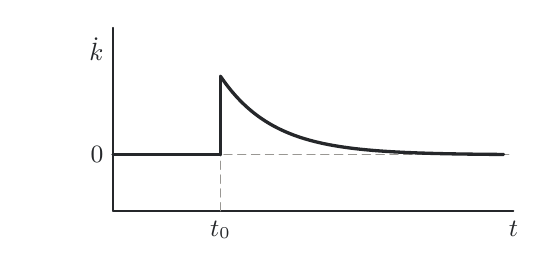
\begin{tikzpicture}[
            x=0.62cm,
            y=0.95cm,
            line cap=round,
            line join=round,
            every node/.style={font=\small},
            declare function={capitalchange(\x)=0.75+1.05*exp(-0.92*(\x-2.20));}
        ]
            \pgfmathsetmacro{\xmax}{8.2}
            \pgfmathsetmacro{\ymax}{2.45}
            \pgfmathsetmacro{\tshock}{2.2}
            \path[use as bounding box] (-1.75,-0.50) rectangle (8.35,\ymax);
            \draw[semithick,DiagramPrimary] (0,0) -- (\xmax,0) node[below] {\(t\)};
            \draw[semithick,DiagramPrimary] (0,0) -- (0,\ymax);
            \node[left] at (0,0.75) {\(0\)};
            \node[below left] at (0,\ymax) {\(\dot{k}\)};
            \draw[densely dashed,DiagramGuide] (0,0.75) -- (\xmax,0.75);
            \draw[DiagramPrimary,very thick] (0,0.75) -- (\tshock,0.75);
            \draw[densely dashed,DiagramGuide] (\tshock,0) -- (\tshock,0.75);
            \draw[DiagramPrimary,very thick] (\tshock,0.75) -- (\tshock,{capitalchange(\tshock)});
            \draw[DiagramPrimary,very thick,domain=2.20:8.0,samples=160]
                plot (\x,{capitalchange(\x)});
            \node[below] at (\tshock,0) {\(t_0\)};
        \end{tikzpicture}
    \end{minipage}

    \vspace{0.65cm}
    \begin{minipage}[t][2.65cm][t]{0.50\textwidth}
        \vspace{0pt}\setstretch{1.3}\raggedright
        储蓄率立即改变了当期投资，但投资无法立即转为资本，所以 \(k\) 不会突变；\(\dot k\) 突变产生了 \(k\) 的路径在 \(t_0\) 出现不光滑点
    \end{minipage}%
    \begin{minipage}[t][2.65cm][t]{0.50\textwidth}
        \vspace{0pt}\raggedleft
        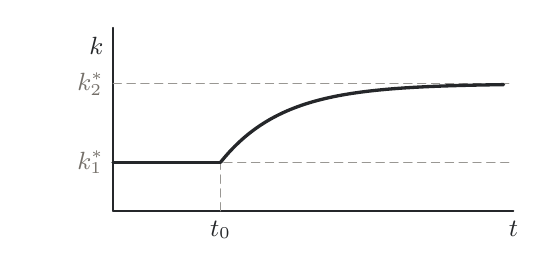
\begin{tikzpicture}[
            x=0.62cm,
            y=0.95cm,
            line cap=round,
            line join=round,
            every node/.style={font=\small},
            declare function={capitalpath(\x)=0.65+1.05*(1-exp(-0.78*(\x-2.20)));}
        ]
            \pgfmathsetmacro{\xmax}{8.2}
            \pgfmathsetmacro{\ymax}{2.45}
            \pgfmathsetmacro{\tshock}{2.2}
            \path[use as bounding box] (-1.75,-0.50) rectangle (8.35,\ymax);
            \draw[semithick,DiagramPrimary] (0,0) -- (\xmax,0) node[below] {\(t\)};
            \draw[semithick,DiagramPrimary] (0,0) -- (0,\ymax);
            \node[below left] at (0,\ymax) {\(k\)};
            \draw[densely dashed,DiagramGuide] (0,0.65) -- (\xmax,0.65);
            \draw[densely dashed,DiagramGuide] (0,1.70) -- (\xmax,1.70);
            \node[left,DiagramAnnotation] at (0,0.65) {\(k_1^*\)};
            \node[left,DiagramAnnotation] at (0,1.70) {\(k_2^*\)};
            \draw[densely dashed,DiagramGuide] (\tshock,0) -- (\tshock,0.65);
            \draw[DiagramPrimary,very thick] (0,0.65) -- (\tshock,0.65);
            \draw[DiagramPrimary,very thick,domain=2.20:8.0,samples=160]
                plot (\x,{capitalpath(\x)});
            \node[below] at (\tshock,0) {\(t_0\)};
        \end{tikzpicture}
    \end{minipage}

    \vspace{0.65cm}
    \begin{minipage}[t][2.65cm][t]{0.50\textwidth}
        \vspace{0pt}\setstretch{1.3}\raggedright
        人均产出是有效人均资本存量的函数，增长率随之突变；但新旧稳态处增长率都是 \(g\)，说明储蓄率的永久变动不会带来持久的增长动力
    \end{minipage}%
    \begin{minipage}[t][2.65cm][t]{0.50\textwidth}
        \vspace{0pt}\raggedleft
        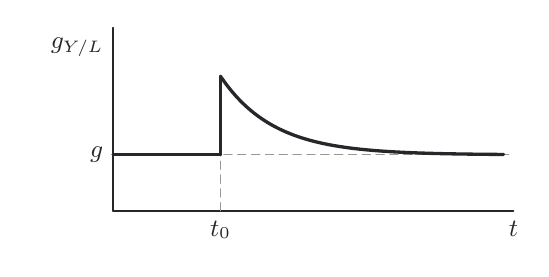
\begin{tikzpicture}[
            x=0.62cm,
            y=0.95cm,
            line cap=round,
            line join=round,
            every node/.style={font=\small},
            declare function={growthpath(\x)=0.75+1.05*exp(-0.92*(\x-2.20));}
        ]
            \pgfmathsetmacro{\xmax}{8.2}
            \pgfmathsetmacro{\ymax}{2.45}
            \pgfmathsetmacro{\tshock}{2.2}
            \path[use as bounding box] (-1.75,-0.50) rectangle (8.35,\ymax);
            \draw[semithick,DiagramPrimary] (0,0) -- (\xmax,0) node[below] {\(t\)};
            \draw[semithick,DiagramPrimary] (0,0) -- (0,\ymax);
            \node[below left] at (0,\ymax) {\(g_{Y/L}\)};
            \node[left] at (0,0.75) {\(g\)};
            \draw[densely dashed,DiagramGuide] (0,0.75) -- (\xmax,0.75);
            \draw[densely dashed,DiagramGuide] (\tshock,0) -- (\tshock,0.75);
            \draw[DiagramPrimary,very thick] (0,0.75) -- (\tshock,0.75);
            \draw[DiagramPrimary,very thick] (\tshock,0.75) -- (\tshock,{growthpath(\tshock)});
            \draw[DiagramPrimary,very thick,domain=2.20:8.0,samples=160]
                plot (\x,{growthpath(\x)});
            \node[below] at (\tshock,0) {\(t_0\)};
        \end{tikzpicture}
    \end{minipage}

    \vspace{0.65cm}
    \begin{minipage}[t][2.65cm][t]{0.50\textwidth}
        \vspace{0pt}\setstretch{1.3}\raggedright
        图像中的斜率是 \(Y/L\) 的增长率，且
        \begingroup
        \setlength{\abovedisplayskip}{2pt}
        \setlength{\belowdisplayskip}{4pt}
        \setlength{\abovedisplayshortskip}{2pt}
        \setlength{\belowdisplayshortskip}{4pt}
        \begin{align*}
            g_{Y/L} = g_A + g_y = g + \dot k\cdot f'\islash f
        \end{align*}
        \endgroup
        \(t_0\) 处随 \(\dot k\) 突变，出现了不光滑点
    \end{minipage}%
    \begin{minipage}[t][2.65cm][t]{0.50\textwidth}
        \vspace{0pt}\raggedleft
        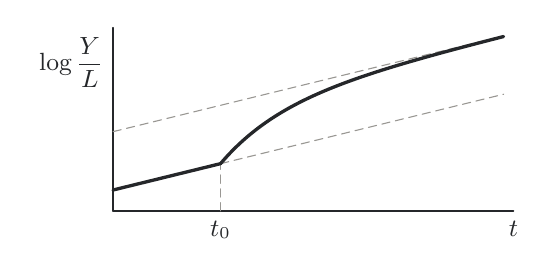
\begin{tikzpicture}[
            x=0.62cm,
            y=0.95cm,
            line cap=round,
            line join=round,
            every node/.style={font=\small},
            declare function={oldtrend(\x)=0.28+0.16*\x; newtrend(\x)=oldtrend(\x)+0.78; outputpath(\x)=oldtrend(\x)+0.78*(1-exp(-0.78*(\x-2.20)));}
        ]
            \pgfmathsetmacro{\xmax}{8.2}
            \pgfmathsetmacro{\ymax}{2.45}
            \pgfmathsetmacro{\tshock}{2.2}
            \path[use as bounding box] (-1.75,-0.50) rectangle (8.35,\ymax);
            \draw[semithick,DiagramPrimary] (0,0) -- (\xmax,0) node[below] {\(t\)};
            \draw[semithick,DiagramPrimary] (0,0) -- (0,\ymax);
            \node[below left] at (0,\ymax) {\(\log\dfrac YL\)};
            \draw[densely dashed,DiagramGuide] (\tshock,0) -- (\tshock,{oldtrend(\tshock)});
            \draw[densely dashed,DiagramGuide,domain=0:8.0,samples=2]
                plot (\x,{oldtrend(\x)});
            \draw[densely dashed,DiagramGuide,domain=0:8.0,samples=2]
                plot (\x,{newtrend(\x)});
            \draw[DiagramPrimary,very thick,domain=0:2.20,samples=2]
                plot (\x,{oldtrend(\x)});
            \draw[DiagramPrimary,very thick,domain=2.20:8.0,samples=160]
                plot (\x,{outputpath(\x)});
            \node[below] at (\tshock,0) {\(t_0\)};
        \end{tikzpicture}
    \end{minipage}

    \vspace{0.65cm}
    \begin{minipage}[t][2.65cm][t]{0.50\textwidth}
        \vspace{0pt}\setstretch{1.3}\raggedright
        不同于资本，储蓄变化会立即改变消费，所以 \(t_0\) 时刻 \(c\) 突变；但最终 \(c\) 会高于还是低于原先，这是不确定的
    \end{minipage}%
    \begin{minipage}[t][2.65cm][t]{0.50\textwidth}
        \vspace{0pt}\raggedleft
        \sidenote{\(c=\bka{1-s}f\bkk\) 对时间求导可知 \(t_0\) 时刻之后消费一定是往上走的而不会下降}
        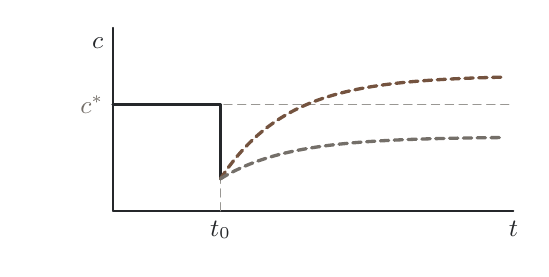
\begin{tikzpicture}[
            x=0.62cm,
            y=0.95cm,
            line cap=round,
            line join=round,
            every node/.style={font=\small},
            declare function={
                consumptionhigh(\x)=0.43+1.38*(1-exp(-0.72*(\x-2.20)));
                consumptionlow(\x)=0.43+0.56*(1-exp(-0.72*(\x-2.20)));
            }
        ]
            \pgfmathsetmacro{\xmax}{8.2}
            \pgfmathsetmacro{\ymax}{2.45}
            \pgfmathsetmacro{\tshock}{2.2}
            \path[use as bounding box] (-1.75,-0.50) rectangle (8.35,\ymax);
            \draw[semithick,DiagramPrimary] (0,0) -- (\xmax,0) node[below] {\(t\)};
            \draw[semithick,DiagramPrimary] (0,0) -- (0,\ymax);
            \node[below left] at (0,\ymax) {\(c\)};
            \draw[densely dashed,DiagramGuide] (0,1.42) -- (\xmax,1.42);
            \node[left,DiagramAnnotation] at (0,1.42) {\(c^*\)};
            \draw[densely dashed,DiagramGuide] (\tshock,0) -- (\tshock,{consumptionhigh(\tshock)});
            \draw[DiagramPrimary,very thick] (0,1.42) -- (\tshock,1.42);
            \draw[DiagramPrimary,very thick] (\tshock,1.42) -- (\tshock,{consumptionhigh(\tshock)});
            \draw[DiagramComparison,very thick,densely dashed,domain=2.20:8.0,samples=160]
                plot (\x,{consumptionhigh(\x)});
            \draw[DiagramAnnotation,very thick,densely dashed,domain=2.20:8.0,samples=160]
                plot (\x,{consumptionlow(\x)});
            \node[below] at (\tshock,0) {\(t_0\)};
        \end{tikzpicture}
    \end{minipage}
    \caption{储蓄率永久上升后的时间路径}
    \label{fig:SolowSavingTransitionPaths}
\end{figure}

\subsection{定量分析}

\noindent\textbf{定量分析：偏导}

\noindent 作图只是帮助我们快速判断参数变动的影响，接下来定量分析不仅能看到变动方向，还能得到变动的线性近似幅度（非真实值），而这一分析由求偏导数给出。

因为我们想看到的是参数对稳态的影响，所以求导从稳态方程开始；同时，稳态方程是关于资本存量的隐函数，那我们就让稳态方程左右两侧 \(k^*\) 对 \(s\) 求偏导数
\begin{align*}
    f\bkkstar+s\,f'\bkkstar\,\frac{\p k^*}{\p s}&=\bka{n+g+\delta}\frac{\p k^*}{\p s}
\end{align*}
整理得
\begin{align*}
    \MathHighlightA{\frac{\p k^*}{\p s}=\frac{f\bkkstar}{\qa{n+g+\delta}-s\,f'\bkkstar}}\sidenote{如果使用隐函数求导公式，能更快得到该结果且不容易算错}
\end{align*}
该结果给出了 \(s\) 变动后 \(k^*\) 的变动方向以及用偏导数线性近似结果，体现出 \(k^*\) 对 \(s\) 有多敏感。上式的符号主要看分母
\begin{align*}
    \bka{n+g+\delta}-s\,f'\bkkstar =  s\bks{\dfrac{f\bkkstar}{k^*}-f'\bkkstar}=s\bka{\n{AC}^*-\n{MC}^*}>0
\end{align*}
所以 \(\p k^*\islash\p s>0\)，\(k^*\) 与 \(s\) 同向变动。

既然已经得到 \(k^*\) 的求导结果，那么 \(y^*\) 的就很容易了
\begin{align*}
    \frac{\p y^*}{\p s} = f'\bkkstar\,\frac{\p k^*}{\p s} = \frac{f'\bkkstar f\bkkstar}{\qa{n+g+\delta}-s\,f'\bkkstar}>0
\end{align*}
\(c^*\) 的求导结果为
\begin{align*}
    \dfrac{\p c^*}{\p s}&=\dfrac{\partial}{\p s}\bks{f\bkkstar-\bka{n+g+\delta}k^*}=\bks{f'\bkkstar-\bka{n+g+\delta}}\dfrac{\p k^*}{\p s}
\end{align*}

\mysec{定量分析：弹性}

\noindent 弹性是经济学更常用的“求导”。因为计算弹性会反复用到储蓄率的表达式，所以我们先从稳态条件中推导出
\begin{align*}
    s=\dfrac{\qa{n+g+\delta}k^*}{f\bkkstar}
\end{align*}

依旧从 \(k^*\) 开始。计算稳态有效人均资本的储蓄率弹性
\begin{align*}
    \dfrac{s}{k^*}\dfrac{\p k^*}{\p s}&=\dfrac{s\,f\bkkstar}{\qa{n+g+\delta}k^*-s\,k^*\,f'\bkkstar}=\dfrac{\MathMarkA{s}\,f\bkkstar}{\MathMarkA{s}\,f\bkkstar-\MathMarkA{s}\,k^*\,f'\bkkstar}\sidenote{推导思路是分子分母都凑出 \(s\) 再同时消去}\\
    &=\dfrac{1}{1-{k^*\,f'\bkkstar}\islash{f\bkkstar}}=\dfrac{1}{1-\alpha_K^*}
\end{align*}
其中 \(\alpha_K^*\) 由 \ref{eq:SolowCapitalShare} 在稳态处定义。同理，稳态有效人均产出的储蓄率弹性为
\begin{align*}
    \dfrac s{y^*}\dfrac{\p y^*}{\p s}&=\dfrac{s\,f'\bkkstar \MathMarkA{f\bkkstar}}{\qa{n+g+\delta}\MathMarkA{f\bkkstar}-s\,f'\bkkstar \MathMarkA{f\bkkstar}}\sidenote{上下同时乘以 \(k^*\)、同时除以 \(\qs{f\bkkstar}^2\)}\\
    &=\dfrac{\MathMarkB{s}\cdot\MathMarkC{k^*\,f'\bkkstar/\,f\bkkstar}}{\MathMarkB{\qa{n+g+\delta}k^*\islash f\bkkstar}-\MathMarkB{s}\cdot\MathMarkC{k^*\,f'\bkkstar/\,f\bkkstar}}=\dfrac{\alpha_K^*}{1-\alpha_K^*}
\end{align*}
以上两个弹性值形式接近并非巧合
\begin{align*}
    \dfrac{s}{y^*}\cdot\dfrac{\p y^*}{\p s}=\dfrac{s}{y^*}\cdot f'\bkkstar\dfrac{\p k^*}{\p s}=\dfrac{k^*\,f'\bkkstar}{f\bkkstar}\cdot\dfrac{s}{k^*}\dfrac{\p k^*}{\p s}=\alpha_K^*\cdot\dfrac{s}{k^*}\dfrac{\p k^*}{\p s}
\end{align*}
在 Cobb--Douglas 情形中，\(\alpha_K\bkk=\alpha\)，无论 \(k^*\) 是多少，上述弹性都是常数。

\mysec{定量分析：其他比较静态}

\noindent 相同的分析方法，以 \(n\) 为例，展示收支平衡线斜率对稳态的影响。直接给出关键结果，具体推导过程留作练习
\begin{align*}
    & \dfrac{\p k^*}{\p n}=-\dfrac{k^*}{\qa{n+g+\delta}-s\,f'\bkkstar}<0\\
    & \frac{n}{y^*}\dfrac{\p y^*}{\p n}=-\dfrac n{n+g+\delta}\cdot\dfrac{\alpha^*_K}{1-\alpha^*_K}<0
\end{align*}

\subsection{收敛速度}\label{subsec:SolowConvergence}

从比较静态分析开始，我们就多次考虑如果脱离了稳态，变量会如何收敛、如何回到平衡增长状态。前文已知经济体受到冲击之后稳态的变动方向和近似幅度，现在来看会以多快速度实现预期的幅度，这被称作\,\term{收敛速度}{speed of convergence}。

这里澄清一件事，\(y\bkt\) 随 \(k\bkt\) 同步变化，所以二者收敛到某个均衡的用时应该是相同的；另一边，\(y^*-y\bko\ne k^*-k\bko\)，那么距离不同、时间相同，速度则不可能相同。实际上，此“速度”非比收敛速度，收敛速度是百分比的瞬时增长率，那么就能理解我们后文会用到 \(y\bkt\) 和 \(k\bkt\) 的收敛速度相同了。

收敛速度实际就是 \(\dot k\bkt\)，我们用一阶泰勒近似，让 \(\dot k\bkt\)\sidenote{\(\dot k\bkt\Leftrightarrow \dot k\bks{k\bkt}\)} 关于 \(k\bkt\) 在稳态 \(k^*\) 附近线性化
\begin{align}
    \dot k &\approx \dot k\bkkstar + \bks{\dfrac{\p \dot k\bkk}{\p k}\biggbar{k=k^*}}\bka{k-k^*}\label{eq:SolowConvergenceSpeed}
    \sidenote{省略时间记号}
\end{align}
等式右侧第一项，在稳态 \(\dot k=0\)；第二项将 \(k-k^*\) 的系数记作 \(-\lambda\) 并作具体计算
\begin{align*}
    \lambda \coloneq -\dfrac{\p \dot k\bkk}{\p k}\biggbar{k=k^*}&=-\bks{s\,f'\bkkstar-\bka{n+g+\delta}}\\
    &=\bka{n+g+\delta}-\dfrac{\bka{n+g+\delta}k^*\,f'\bkkstar}{f\bkkstar}\\
    &=\MathHighlightA{\bka{n+g+\delta}\bka{1-\alpha^*_K}}
\end{align*}
代回 \ref{eq:SolowConvergenceSpeed}，然后解微分方程得有效人均资本的路径
\begin{align*}
    \dot k\bkt\approx-\lambda\bks{k\bkt-k^*}\means k\bkt\approx k^*+\bks{k\bko-k^*}e^{-\lambda t}
    \sidenote{从 \(-\lambda\) 出现在指数中作为时间的系数，就可知它是瞬时变化率}
\end{align*}

前文说过 \(y\bkt\) 和 \(k\bkt\) 有相同的收敛速度，那么能直接写出
\begin{align*}
    y\bkt\approx y^*+\bks{y\bko-y^*}e^{-\lambda t}
\end{align*}


% \BeginChapterAppendix

% \section{离散与连续}\label{sec:SolowDiscreteContinuous}

% \section{零散推导}\label{sec:SolowMiscDerivations}

% \myskip
% \mysec{规模报酬不变获得零利润}

% 利用反证法，假设厂商获得非零最大利润，即
% \begin{align*}
%     \pi_{\text{max}}=P\,F\bka{K,L}-r\,K-w\,L>0
% \end{align*}
% 将要素投入量扩大 \(\lambda>1\) 倍，根据规模报酬不变性质可得
% \begin{align*}
%     P\,F\bka{\lambda\,L,\lambda\,K} -w\,\lambda\,L-r\lambda\,K = \lambda\,P\,F\bka{L,K} -w\,\lambda\,L-r\,\lambda\,K = \lambda\,\pi _{\text{max}}>\pi_{\text{max}}
% \end{align*}
% 说明通过扩大生产，厂商可以获得更大的利润，与假设相悖。于是，厂商最大利润为零。

\FinishStandaloneChapter
